\documentclass[a4paper,11pt,twoside]{article}

% =========================================================================
%  Ecuaciones Diferenciales — Tema 4: EDO lineales de orden superior.
%  Parte I: estructura de las soluciones, coeficientes constantes,
%  variación de constantes y funciones de Green.
%
%  Compilación:   latexmk main.tex      (LuaLaTeX + biber)
%  Imagen de portada: python3 scripts/generar_portada.py   (ya incluida)
%  Datos de las gráficas: python3 scripts/generar_datos.py  (ya incluidos)
% =========================================================================
% =========================================================================
%  Ecuaciones Diferenciales — Tema 4: EDO lineales de orden superior.
%  Parte I: estructura de las soluciones, coeficientes constantes,
%  variación de constantes y funciones de Green.
%
%  Estilo: artículo matemático sobre fondo oscuro (texto claro en Computer
%  Modern, como en las láminas de análisis complejo de referencia), con
%  enunciados numerados por sección, cajas con pestaña de título para
%  definiciones y teoremas y figuras TikZ/pgfplots adaptadas al fondo negro.
% =========================================================================

% --- IDIOMA Y CODIFICACIÓN ------------------------------------------------
% Se compila con LuaLaTeX (memoria dinámica para las superficies 3D);
% con pdfLaTeX funciona igualmente reduciendo la resolución de esas figuras.
\usepackage{iftex}
\ifPDFTeX
  \usepackage[utf8]{inputenc}
  \usepackage[T1]{fontenc}
  \usepackage{lmodern}
\else
  \usepackage{fontspec}   % Latin Modern (Computer Modern OpenType) por defecto
\fi
\usepackage[spanish,es-tabla,es-nodecimaldot,es-noshorthands,es-lcroman]{babel}

% --- TIPOGRAFÍA (Latin Modern = Computer Modern vectorial) ----------------
\usepackage[final]{microtype}
\linespread{1.06}
\emergencystretch=2em

% --- MATEMÁTICAS -------------------------------------------------------------
\usepackage{amsmath, amssymb, mathtools}
\usepackage{bm}
\usepackage{mathrsfs}
\usepackage{cancel}

% --- PÁGINA -----------------------------------------------------------------
\usepackage[a4paper, top=2.9cm, bottom=2.7cm, left=2.7cm, right=2.7cm,
            headsep=0.9cm, headheight=22pt]{geometry}
\usepackage{graphicx}

% --- PALETA OSCURA ------------------------------------------------------------
\usepackage[table]{xcolor}
\definecolor{fondo}{HTML}{000000}      % fondo de página (negro puro)
\definecolor{texto}{HTML}{ECECEC}      % texto principal (blanco suave)
\definecolor{blanco}{HTML}{FFFFFF}
\definecolor{negro}{HTML}{000000}
\definecolor{gris}{HTML}{9CA0A8}       % texto secundario, ejes
\definecolor{grismedio}{HTML}{5B5F67}  % reglas, marcos tenues
\definecolor{grisoscuro}{HTML}{2E3036} % rejillas, divisiones
\definecolor{cajafondo}{HTML}{0E1014}  % interior de las cajas
\definecolor{cian}{HTML}{20B4CE}       % definiciones y acento principal
\definecolor{cianclaro}{HTML}{7FDBEA}  % enlaces
\definecolor{violeta}{HTML}{A48BFA}    % teoremas, proposiciones, lemas
\definecolor{ambar}{HTML}{F4B740}      % resultados clave, receta
\definecolor{magenta}{HTML}{E5579D}
\definecolor{verde}{HTML}{4FD68A}
\definecolor{naranja}{HTML}{FA8F45}
\definecolor{rojo}{HTML}{F25F5C}

% Página negra y texto claro. Se fija en el preámbulo para que el color
% «por defecto» (el que restauran flotantes, notas, cabeceras...) sea el claro.
\pagecolor{fondo}
\color{texto}

% --- GRÁFICOS -----------------------------------------------------------------
\usepackage{tikz}
\usetikzlibrary{arrows.meta, calc, positioning, decorations.pathmorphing,
                decorations.markings, decorations.pathreplacing, patterns,
                shapes.geometric, shapes.misc, fit, backgrounds, shadings,
                fadings, intersections}
\usepackage{pgfplots}
\pgfplotsset{compat=1.18}
\usepgfplotslibrary{colormaps, fillbetween, groupplots}

% --- LISTAS, TABLAS, CABECERAS ----------------------------------------------
\usepackage{booktabs}
\usepackage{array}
\usepackage{multirow}
\usepackage{enumitem}
\setlist[itemize]{leftmargin=1.6em, itemsep=2pt, topsep=4pt,
                  label={\color{cian}\scriptsize$\blacktriangleright$}}
\setlist[enumerate]{leftmargin=1.9em, itemsep=2pt, topsep=4pt}
\arrayrulecolor{grismedio}

\usepackage{fancyhdr}
\pagestyle{fancy}
\fancyhf{}
\fancyhead[LE]{\small\color{gris}\thepage\hfill\scshape Ecuaciones Diferenciales}
\fancyhead[RO]{\small\color{gris}\scshape Tema 4\,·\,EDO lineales de orden superior\hfill\upshape\thepage}
\fancyhead[LO,RE]{}
\renewcommand{\headrulewidth}{0.3pt}
\renewcommand{\headrule}{\hbox to\headwidth{\color{grisoscuro}\leaders\hrule height \headrulewidth\hfill}}
\fancypagestyle{plain}{\fancyhf{}\renewcommand{\headrulewidth}{0pt}%
  \fancyfoot[C]{\small\color{gris}\thepage}}

% --- TÍTULOS DE SECCIÓN -----------------------------------------------------
\usepackage{titlesec}
\titleformat{\section}[block]
  {\normalfont\Large\bfseries\color{blanco}}
  {\color{cian}\thesection}{0.9em}{}
  [{\vspace{3pt}\color{grisoscuro}\titlerule[0.5pt]}]
\titlespacing*{\section}{0pt}{4.2ex plus 1ex minus .4ex}{2.2ex plus .4ex}
\titleformat{\subsection}[block]
  {\normalfont\large\bfseries\color{blanco}}
  {\color{cian}\thesubsection}{0.8em}{}
\titlespacing*{\subsection}{0pt}{3.2ex plus 1ex minus .4ex}{1.4ex plus .3ex}
\titleformat{\paragraph}[runin]
  {\normalfont\bfseries\color{blanco}}{}{0pt}{}[.]
\titlespacing*{\paragraph}{0pt}{1.6ex plus .5ex}{0.6em}
% Evita títulos huérfanos al pie de página
\usepackage{needspace}
\usepackage{placeins}
\usepackage{etoolbox}
\AtBeginDocument{%
  \pretocmd{\section}{\needspace{9\baselineskip}}{}{}%
  \pretocmd{\subsection}{\needspace{6\baselineskip}}{}{}}
\setcounter{secnumdepth}{2}
\setcounter{tocdepth}{2}

% --- ÍNDICE -------------------------------------------------------------------
\usepackage{tocloft}
\renewcommand{\cfttoctitlefont}{\normalfont\Large\bfseries\color{blanco}}
\renewcommand{\cftsecfont}{\bfseries\color{blanco}}
\renewcommand{\cftsecpagefont}{\bfseries\color{cian}}
\renewcommand{\cftsubsecfont}{\color{texto}}
\renewcommand{\cftsubsecpagefont}{\color{gris}}
\renewcommand{\cftsecleader}{\color{grismedio}\cftdotfill{\cftdotsep}}
\renewcommand{\cftsubsecleader}{\color{grisoscuro}\cftdotfill{\cftdotsep}}
\setlength{\cftbeforesecskip}{6pt}
\renewcommand{\contentsname}{Índice}

% --- ENLACES Y REFERENCIAS CRUZADAS ----------------------------------------
\usepackage[colorlinks=true, linkcolor=cianclaro, citecolor=ambar,
            urlcolor=cianclaro, plainpages=false, pdfusetitle=false,
            pdftitle={Tema 4. EDO lineales de orden superior y funciones de Green},
            pdfauthor={Daniel Martín Guerrero},
            pdfsubject={Ecuaciones Diferenciales},
            bookmarksnumbered=true]{hyperref}
\usepackage{amsthm}
\usepackage[spanish,nameinlink]{cleveref}   % tras amsthm y hyperref

% --- BIBLIOGRAFÍA -----------------------------------------------------------
\usepackage{csquotes}
\usepackage[backend=biber, style=numeric, sorting=none, giveninits=true,
            maxbibnames=6, minbibnames=3, doi=false, url=false,
            isbn=false]{biblatex}
\addbibresource{referencias.bib}
\renewcommand*{\bibfont}{\small}
\setlength{\bibitemsep}{4pt}

% --- PIES DE FIGURA -------------------------------------------------------
\usepackage[font={small,color=texto}, labelfont={sc,color=cian},
            labelsep=period, margin=0.4cm, justification=justified,
            skip=8pt]{caption}
\usepackage{subcaption}
\numberwithin{equation}{section}
\numberwithin{figure}{section}
\numberwithin{table}{section}

% =========================================================================
%               NOTACIÓN Y MACROS
% =========================================================================
\newcommand{\dif}{\mathrm{d}}
\newcommand{\eul}{\mathrm{e}}
\newcommand{\iu}{\mathrm{i}}
\newcommand{\R}{\mathbb{R}}
\newcommand{\C}{\mathbb{C}}
\newcommand{\N}{\mathbb{N}}
\newcommand{\Z}{\mathbb{Z}}
\newcommand{\abs}[1]{\lvert #1\rvert}
\newcommand{\Abs}[1]{\left\lvert #1\right\rvert}
\newcommand{\defeq}{\mathrel{\overset{\mathrm{def}}{=}}}
\newcommand{\Cinf}{\mathcal{C}^{\infty}}
\newcommand{\Com}{\mathcal{C}^{\omega}}           % funciones analíticas reales
\newcommand{\disco}[2]{D(#1,#2)}                  % disco abierto
\newcommand{\dd}[2]{\frac{\dif #1}{\dif #2}}
\newcommand{\ddd}[2]{\frac{\dif^{2} #1}{\dif #2^{2}}}
\newcommand{\serie}[3][n]{\sum_{#1=#2}^{\infty}#3}
\DeclareMathOperator{\sen}{sen}
\DeclareMathOperator{\senh}{senh}
\DeclareMathOperator{\artanh}{artanh}
\DeclareMathOperator{\dist}{dist}
\DeclareMathOperator{\Real}{Re}
\DeclareMathOperator{\Imag}{Im}
\DeclareMathOperator{\Arg}{arg}
\DeclareMathOperator{\ord}{ord}
\DeclareMathOperator{\Ai}{Ai}
\DeclareMathOperator{\Bi}{Bi}
\renewcommand{\sin}{\sen}
\newcommand{\Heav}{\Theta}
\newcommand{\Lop}{\mathcal{L}}                     % operador diferencial lineal
\newcommand{\Dop}{D}                               % D = d/dx
\newcommand{\yv}{\hat{\bm y}}                      % vector (y_1,...,y_n)^T
\newcommand{\kv}{\bm{k}}
\newcommand{\bv}{\bm{b}}
\newcommand{\en}{\bm{e}_n}
\newcommand{\T}{\mathsf{T}}
\DeclareMathOperator{\Ker}{ker}
\DeclareMathOperator{\spanop}{span}
\newcommand{\nota}[1]{\textcolor{gris}{#1}}        % texto secundario
\newcommand{\resalta}[1]{\textcolor{blanco}{\bfseries #1}}
% Llaves horizontales en color tenue
\newcommand{\ubr}[2]{\underbrace{#1}_{\textcolor{gris}{#2}}}

% =========================================================================
%        ENTORNOS FORMALES
% =========================================================================
\usepackage[most]{tcolorbox}

% Contador común a todos los enunciados (numeración «sección.n»)
\newcounter{enunciado}[section]
\renewcommand{\theenunciado}{\thesection.\arabic{enunciado}}

% --- Cajas con pestaña (definiciones, teoremas, resultados) -------------------
% #1 color del marco, #2 rótulo completo
\tcbset{
  caja/.style={enhanced, colback=cajafondo, colupper=texto,
    colframe=#1, boxrule=0.7pt, arc=2.5pt, outer arc=2.5pt,
    left=10pt, right=10pt, top=11pt, bottom=8pt,
    before skip=16pt plus 2pt, after skip=14pt plus 2pt,
    attach boxed title to top left={yshift*=-\tcboxedtitleheight/2, xshift=10pt},
    boxed title style={colback=#1, colframe=#1, arc=2pt, outer arc=2pt,
                       boxrule=0pt, left=5pt, right=5pt, top=1.5pt, bottom=1.5pt},
    fonttitle=\sffamily\bfseries\small, coltitle=negro},
}
% Constructor: \cajaenunciado{nombre}{Rótulo}{color}{estilo cuerpo}
\makeatletter
\newcommand{\cajaenunciado}[4]{%
  \newcounter{#1}%
  \expandafter\def\csname the#1\endcsname{\theenunciado}%
  \expandafter\def\csname theH#1\endcsname{#1.\arabic{#1}}%
  \newtcolorbox{tcb@#1}[1]{caja=#3,
      title={#2~\theenunciado\ifx\relax##1\relax\else\ \textnormal{\sffamily(##1)}\fi}}%
  \newenvironment{#1}[1][]%
    {\par\stepcounter{enunciado}\refstepcounter{#1}%
     \begin{tcb@#1}{##1}#4\ignorespaces}%
    {\end{tcb@#1}}%
}
\makeatother
\cajaenunciado{definicion}{Definición}{cian}{\normalfont}
\cajaenunciado{teorema}{Teorema}{violeta}{\itshape}
\cajaenunciado{proposicion}{Proposición}{violeta}{\itshape}
\cajaenunciado{lema}{Lema}{violeta}{\itshape}
\cajaenunciado{corolario}{Corolario}{violeta}{\itshape}
\cajaenunciado{resultado}{Resultado}{ambar}{\normalfont}

% Caja de método (receta), sin numerar
\newtcolorbox{metodo}[1][Método]{caja=ambar, title={#1}}

% --- Enunciados sin caja (ejemplos, observaciones, notación) -----------------
\newtheoremstyle{ejemplo}{12pt}{10pt}{\normalfont}{}%
  {\bfseries\color{cian}}{.}{0.6em}%
  {\thmname{#1}\thmnumber{ #2}\thmnote{\normalfont\color{gris}\ (#3)}}
\newtheoremstyle{observacion}{10pt}{10pt}{\normalfont}{}%
  {\itshape\bfseries\color{violeta}}{.}{0.6em}%
  {\thmname{#1}\thmnumber{ #2}\thmnote{\normalfont\itshape\color{gris}\ (#3)}}
\theoremstyle{ejemplo}
\newtheorem{ejemplo}[enunciado]{Ejemplo}
\newtheorem{notacion}[enunciado]{Notación}
\theoremstyle{observacion}
\newtheorem{observacion}[enunciado]{Observación}

% Demostraciones
\renewcommand{\qedsymbol}{\textcolor{gris}{$\blacksquare$}}
\makeatletter
\renewenvironment{proof}[1][\proofname]{\par
  \pushQED{\qed}\normalfont\topsep6\p@\@plus6\p@\relax
  \trivlist\item[\hskip\labelsep\itshape\bfseries\color{gris}#1\@addpunct{.}]\ignorespaces
}{\popQED\endtrivlist\@endpefalse}
\makeatother
\newenvironment{esbozo}{\begin{proof}[Esbozo de la demostración]}{\end{proof}}

% Notas al margen del discurso: «idea», recuadro tenue con barra lateral
\newtcolorbox{idea}[1][Idea]{enhanced, breakable, colback=cajafondo, colupper=texto,
  frame hidden, borderline west={2pt}{0pt}{cian!80}, arc=0pt,
  left=10pt, right=8pt, top=6pt, bottom=6pt, before skip=12pt, after skip=12pt,
  fontupper=\normalfont,
  before upper={{\sffamily\bfseries\small\color{cian}#1.}\ }}

\crefname{definicion}{definición}{definiciones}
\Crefname{definicion}{Definición}{Definiciones}
\crefname{teorema}{teorema}{teoremas}
\Crefname{teorema}{Teorema}{Teoremas}
\crefname{proposicion}{proposición}{proposiciones}
\Crefname{proposicion}{Proposición}{Proposiciones}
\crefname{lema}{lema}{lemas}
\Crefname{lema}{Lema}{Lemas}
\crefname{corolario}{corolario}{corolarios}
\Crefname{corolario}{Corolario}{Corolarios}
\crefname{resultado}{resultado}{resultados}
\Crefname{resultado}{Resultado}{Resultados}
\crefname{ejemplo}{ejemplo}{ejemplos}
\Crefname{ejemplo}{Ejemplo}{Ejemplos}
\crefname{observacion}{observación}{observaciones}
\Crefname{observacion}{Observación}{Observaciones}
\crefname{notacion}{notación}{notaciones}
\Crefname{notacion}{Notación}{Notaciones}
\crefname{section}{sección}{secciones}
\Crefname{section}{Sección}{Secciones}
\crefname{subsection}{apartado}{apartados}
\Crefname{subsection}{Apartado}{Apartados}
\crefname{figure}{figura}{figuras}
\Crefname{figure}{Figura}{Figuras}
\crefname{table}{tabla}{tablas}
\Crefname{table}{Tabla}{Tablas}
\crefname{equation}{ecuación}{ecuaciones}
\Crefname{equation}{Ecuación}{Ecuaciones}
\crefformat{equation}{(#2#1#3)}
\Crefformat{equation}{Ecuación~(#2#1#3)}
\crefrangeformat{equation}{(#3#1#4)--(#5#2#6)}
\crefmultiformat{equation}{(#2#1#3)}{ y~(#2#1#3)}{, (#2#1#3)}{ y~(#2#1#3)}

% Modo rápido: si existe el fichero vacío «rapido.flag», las superficies y
% retratos de fase se generan con baja resolución (compilación en segundos).
\newif\ifrapido
\IfFileExists{rapido.flag}{\rapidotrue}{\rapidofalse}
\ifrapido
  \def\resPx{24}\def\resPy{34}\def\resF{41}
\else
  \def\resPx{85}\def\resPy{131}\def\resF{141}
\fi

% =========================================================================
%        ESTILOS GRÁFICOS COMUNES
% =========================================================================
% =========================================================================
%  Estilos gráficos comunes (TikZ / pgfplots) para fondo negro
% =========================================================================

% --- Mapa de colores «arcoíris» para coloreado por fase (dominio complejo) ---
% Recorre el círculo cromático completo: el color codifica arg f(z) en (-pi,pi].
\pgfplotsset{colormap={fase}{
  rgb255=(255,40,60) rgb255=(255,150,20) rgb255=(250,230,40)
  rgb255=(60,220,90) rgb255=(30,200,230) rgb255=(60,90,255)
  rgb255=(190,60,240) rgb255=(255,40,60)}}

% --- Estilos TikZ generales ------------------------------------------------
\tikzset{
  >=Stealth,
  every picture/.append style={line cap=round, line join=round},
  eje/.style={-{Stealth[length=5pt,width=4pt]}, line width=0.6pt, gris},
  ejeclaro/.style={-{Stealth[length=5pt,width=4pt]}, line width=0.7pt, texto},
  fino/.style={line width=0.4pt, grismedio},
  guia/.style={densely dashed, line width=0.45pt, grismedio},
  punteado/.style={densely dotted, line width=0.6pt, gris},
  etiq/.style={font=\small, text=texto},
  etiqgris/.style={font=\footnotesize, text=gris},
  polo/.style={cross out, draw=rojo, line width=1.1pt, minimum size=6pt, inner sep=0pt},
  punto/.style={circle, fill=blanco, inner sep=0pt, minimum size=4pt},
  puntocian/.style={circle, fill=cian, inner sep=0pt, minimum size=4.5pt},
  orienta/.style={decoration={markings, mark=at position #1 with
     {\arrow{Stealth[length=6pt,width=5pt]}}}, postaction={decorate}},
  orienta/.default=0.55,
  nodo/.style={draw=grismedio, fill=cajafondo, rounded corners=2pt,
     line width=0.5pt, inner xsep=6pt, inner ysep=4pt, font=\small, text=texto},
  nodocian/.style={nodo, draw=cian},
  nodoambar/.style={nodo, draw=ambar},
  nodovioleta/.style={nodo, draw=violeta},
  flecha/.style={-{Stealth[length=5pt,width=4.5pt]}, line width=0.6pt, gris},
}

% --- Estilo base de ejes pgfplots en oscuro ----------------------------------
\pgfplotsset{
  oscuro/.style={
    axis background/.style={fill=fondo},
    tick label style={font=\scriptsize, text=gris},
    label style={font=\small, text=texto},
    title style={font=\small, text=texto},
    axis line style={grismedio, line width=0.5pt},
    every tick/.style={grismedio},
    major tick length=3pt,
    grid=major, grid style={grisoscuro, line width=0.35pt},
    legend style={font=\scriptsize, draw=grisoscuro, fill=cajafondo,
                  text=texto, rounded corners=1.5pt, inner sep=3pt,
                  row sep=1pt},
    legend cell align=left,
    /pgf/number format/use comma,
    /pgf/number format/1000 sep={},
    unbounded coords=jump,
  },
  % Ejes cruzados por el origen (estilo «pizarra»)
  cruz/.style={oscuro, axis lines=middle, grid=none,
    axis line style={gris, line width=0.6pt,
      -{Stealth[length=5pt,width=4pt]}},
    xlabel style={anchor=west, font=\small},
    ylabel style={anchor=south, font=\small},
  },
  superficie/.style={
    tick label style={font=\scriptsize, text=gris},
    label style={font=\small, text=texto},
    axis line style={grismedio}, every tick/.style={grismedio},
    grid=none, colormap name=fase, shader=interp,
    /pgf/number format/use comma,
  },
  % Curvas
  c1/.style={line width=1.15pt, cian},
  c2/.style={line width=1.15pt, magenta},
  c3/.style={line width=1.15pt, ambar},
  c4/.style={line width=1.15pt, verde},
  c5/.style={line width=1.15pt, violeta},
  c6/.style={line width=1.15pt, naranja},
}


% Escala progresiva para familias de curvas (azul -> violeta)
\definecolor{cm1}{RGB}{60,90,255}
\definecolor{cm2}{RGB}{45,145,240}
\definecolor{cm3}{RGB}{30,200,230}
\definecolor{cm4}{RGB}{60,220,90}
\definecolor{cm5}{RGB}{250,230,40}
\definecolor{cm6}{RGB}{255,150,20}
\definecolor{cm7}{RGB}{255,40,60}
\definecolor{cm8}{RGB}{190,60,240}



% =========================================================================
%                     VARIABLES PARA LA PORTADA
% =========================================================================
\newcommand{\Universidad}{Universidad de Salamanca}
\newcommand{\Facultad}{Facultad de Ciencias}
\newcommand{\Titulacion}{Grado en Física}
\newcommand{\Asignatura}{Ecuaciones Diferenciales}
\newcommand{\NumTema}{Tema 4}
\newcommand{\TituloTema}{EDO lineales\\de orden superior}
\newcommand{\SubtituloTema}{Parte I\,·\,Estructura de las soluciones, coeficientes constantes\\y funciones de Green}
\newcommand{\tipotrabajo}{Apuntes formalizados}
\newcommand{\miNombre}{Daniel Martín Guerrero}
\newcommand{\miProfesorado}{\begin{tabular}{@{}c@{}}Pilar García Estévez\\José Beltrán Jiménez\\María Pérez Garrote\end{tabular}}
\newcommand{\miUbicacion}{Salamanca, curso 2026/2027}

% =========================================================================
%                                DOCUMENTO
% =========================================================================
\begin{document}

% --- PORTADA ----------------------------------------------------------------
\pagenumbering{alph}
%%%%%%%%%%%%%%%%%%%%%%%%%%%%%%%%%%%%%%%%%%%%%%%%%%%%%%%%%%%%%%%%%%%%%%%%
% Portada oscura: identificación institucional, título, imagen de la
% superposición de respuestas a impulsos (scripts/generar_portada.py) y
% datos de autoría.
%%%%%%%%%%%%%%%%%%%%%%%%%%%%%%%%%%%%%%%%%%%%%%%%%%%%%%%%%%%%%%%%%%%%%%%%
\begin{titlepage}
\thispagestyle{empty}
\begin{tikzpicture}[remember picture, overlay]
  \coordinate (O) at (current page.south west);
  \coordinate (C) at ($(O)+(10.5cm,0)$);

  % Logotipo y cabecera institucional
  \node[anchor=north, inner sep=0] at ($(C)+(0,27.6cm)$)
    {
\includegraphics[height=1.45cm]{logo_usal_blanco.png}};
  \draw[grismedio, line width=0.35pt] ($(O)+(3.0cm,25.6cm)$) -- ($(O)+(18.0cm,25.6cm)$);
  \node[anchor=north, align=center, inner sep=0] at ($(C)+(0,25.15cm)$)
    {{\color{gris}\scshape\small\textls[140]{\Facultad\ \ ·\ \ \Titulacion}}};

  % Asignatura, tema y título
  \node[anchor=north, align=center, inner sep=0, text width=16cm] at ($(C)+(0,23.3cm)$)
    {{\color{cian}\scshape\large\textls[180]{\Asignatura}}\\[6pt]
     {\color{gris}\scshape\normalsize\textls[140]{\NumTema}}\\[20pt]
     {\color{blanco}\fontsize{30}{37}\selectfont\bfseries\TituloTema}\\[14pt]
     {\color{cian}\rule{3.2cm}{0.7pt}}\\[12pt]
     {\color{texto}\itshape\large\SubtituloTema}};

  % Respuestas a impulsos (en cascada) y su superposición
  \node[anchor=center, inner sep=0] at ($(C)+(0,10.6cm)$)
    {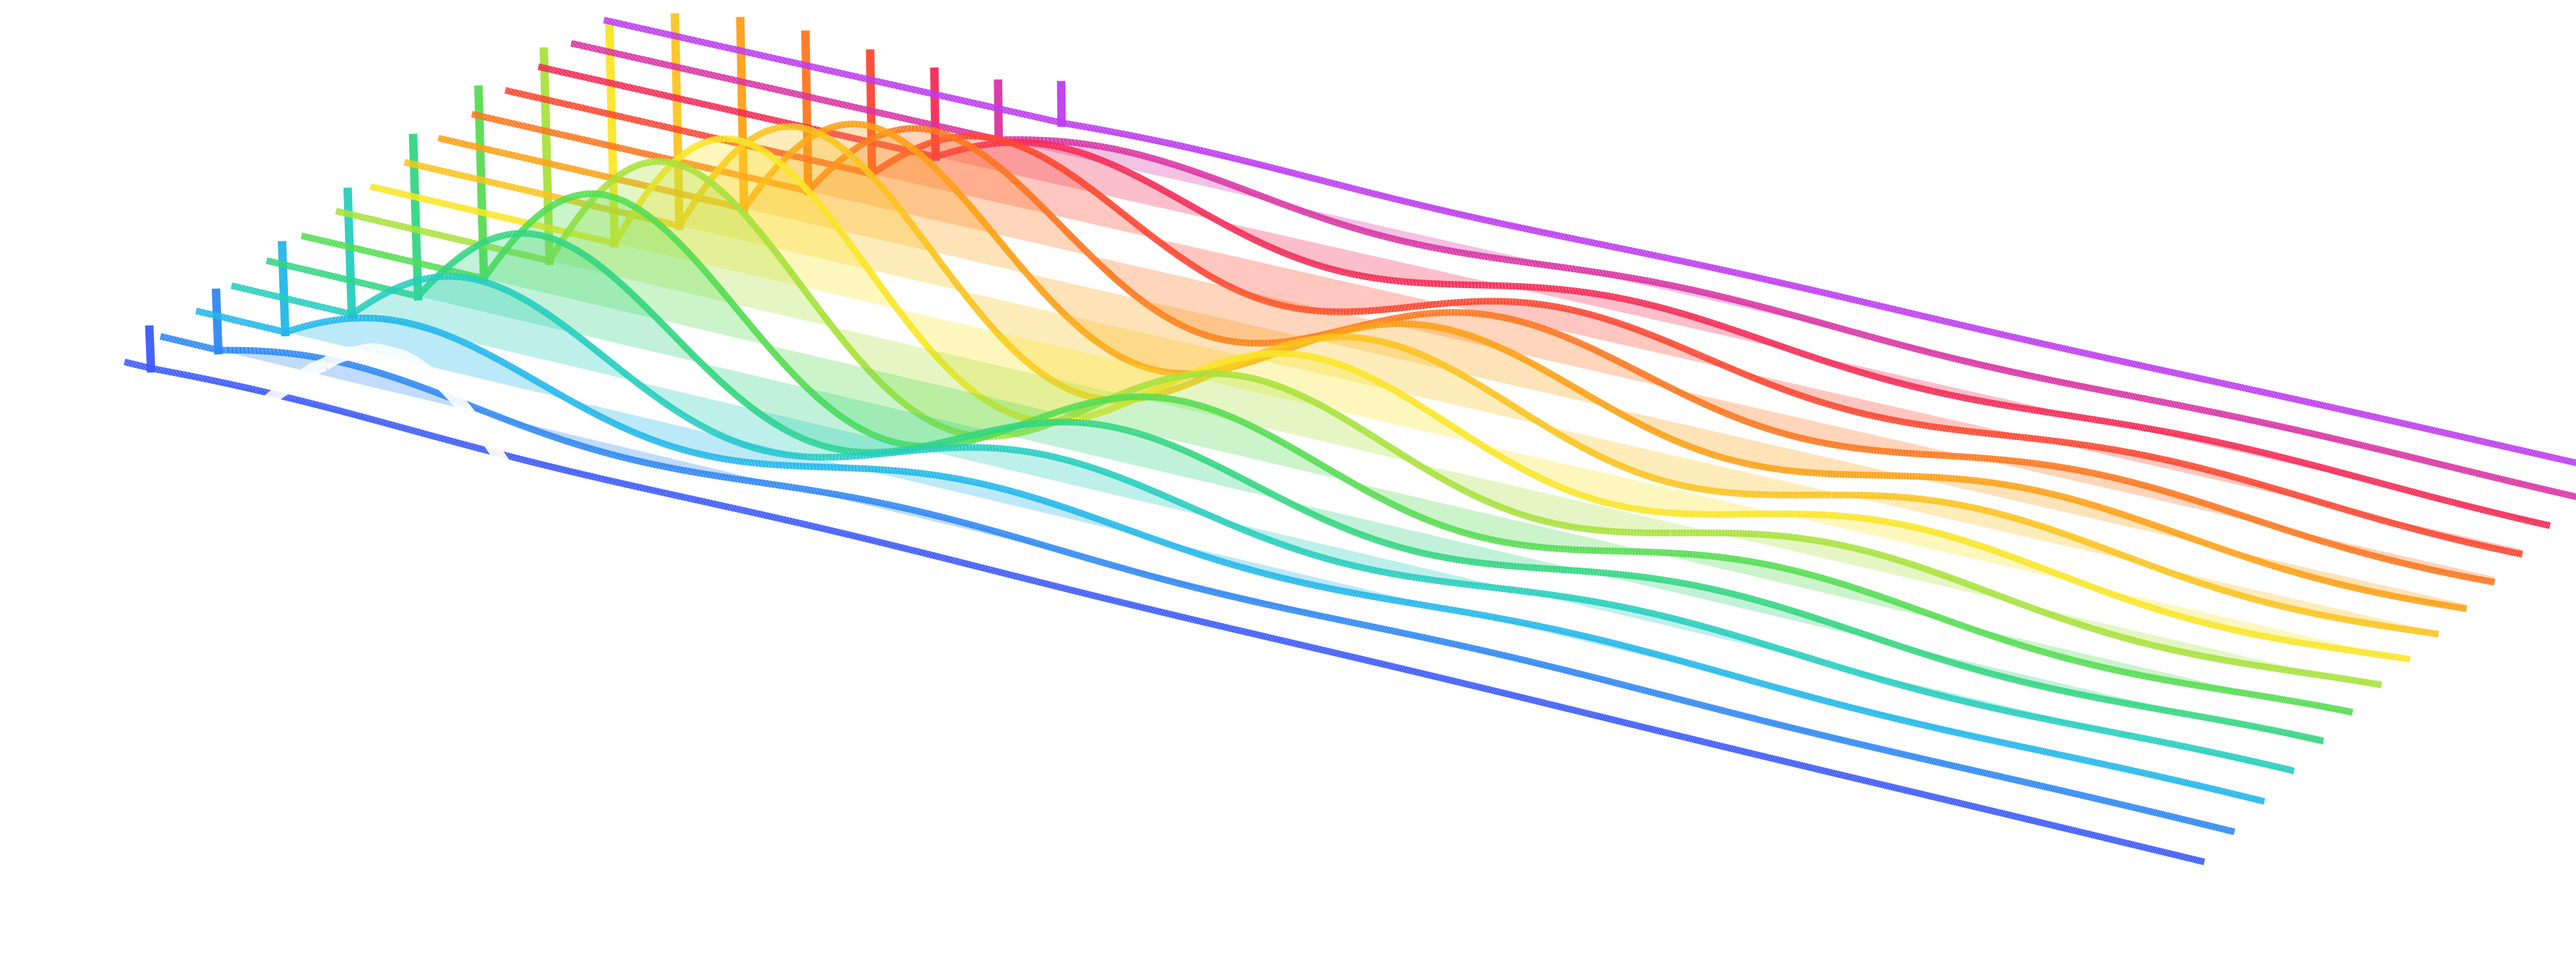
\includegraphics[width=16.4cm]{figuras/portada_superficie.png}};

  % Epígrafe: la función de Green y la solución como superposición
  \node[anchor=north, align=center, inner sep=0] at ($(C)+(0,6.4cm)$)
    {\color{texto}$\displaystyle
      \Lop_x\,G(x,\tilde x)=\delta(x-\tilde x),\qquad
      y_p(x)=\int G(x,\tilde x)\,b(\tilde x)\,\dif\tilde x$};

  % Autoría, profesorado, lugar y curso
  \draw[grismedio, line width=0.35pt] ($(O)+(3.0cm,4.2cm)$) -- ($(O)+(18.0cm,4.2cm)$);
  \node[anchor=north west, inner sep=0, align=left] at ($(O)+(3.0cm,3.75cm)$)
    {{\scshape\small\color{cian}\textls[100]{Autor}}\\[3pt]
     {\large\color{blanco}\miNombre}};
  \node[anchor=north, inner sep=0, align=center] at ($(C)+(0,3.75cm)$)
    {{\scshape\small\color{cian}\textls[100]{Profesorado}}\\[3pt]
     {\small\color{texto}\miProfesorado}};
  \node[anchor=north east, inner sep=0, align=right] at ($(O)+(18.0cm,3.75cm)$)
    {{\scshape\small\color{cian}\textls[100]{\tipotrabajo}}\\[3pt]
     {\color{gris}\miUbicacion}};
\end{tikzpicture}
\end{titlepage}

\clearpage
\pagenumbering{arabic}
\setcounter{page}{1}

% --- CABECERA DEL ARTÍCULO ------------------------------------------------
\thispagestyle{plain}
\begin{center}
  {\color{gris}\scshape\small\textls[120]{\Asignatura\ \,·\ \,\NumTema}}\par\vspace{10pt}
  {\color{blanco}\LARGE\bfseries Ecuaciones diferenciales lineales\\[3pt]
   de orden superior y funciones de Green}\par\vspace{12pt}
  {\color{cian}\rule{2.8cm}{0.6pt}}\par\vspace{10pt}
  {\large\color{texto}\miNombre}\par\vspace{2pt}
  {\small\itshape\color{gris}\Titulacion, \Facultad, \Universidad}\par
\end{center}
\vspace{14pt}

\begin{center}
\begin{minipage}{0.86\textwidth}
\small
{\scshape\color{cian}Resumen.}\ \
Estudiamos la ecuación lineal de orden $n$
$\Lop[y]=a_n(x)\,y^{(n)}+\dots+a_0(x)\,y=b(x)$. Toda la teoría descansa en la
linealidad de $\Lop$: de ella se siguen que las soluciones de la homogénea
forman un espacio vectorial de dimensión $n$ ---lo que demostramos
identificándolo con el espacio de datos iniciales--- y que la solución
general es la suma de la homogénea y una particular. Para coeficientes
constantes construimos una base del núcleo factorizando $\Lop$ como
polinomio en $D=\dif/\dif x$, incluido el caso de raíces múltiples, que
resolvemos con un lema de conjugación por la exponencial. Para la
particular deducimos la fórmula matricial de variación de las constantes
y mostramos que coincide con el método de la función de Green, la
respuesta del sistema a un impulso unitario, que permite escribir la
solución como superposición de respuestas a fuentes puntuales.

\medskip
{\scshape\color{cian}Palabras clave.}\ \
operador lineal, sistema fundamental, wronskiano, polinomio
característico, raíces múltiples, variación de las constantes, función de
Green, delta de Dirac, causalidad.

\medskip
{\scshape\color{cian}MSC 2020.}\ \ 34A30, 34A05, 34B27.
\end{minipage}
\end{center}

\clearpage
{\hypersetup{linkcolor=texto}\tableofcontents}
\clearpage

% =========================================================================
\section{Planteamiento y estructura de la solución}\label{sec:estructura}
% =========================================================================

Todo el tema descansa sobre una sola propiedad: el operador diferencial es
\emph{lineal}. De ella se siguen tres hechos: que la solución general es
«homogénea más particular», que las soluciones de la homogénea forman un
espacio vectorial de dimensión $n$, y que una fuente complicada puede
descomponerse en impulsos elementales cuyas respuestas se suman
(\cref{sec:green}).

% -------------------------------------------------------------------------
\subsection{El operador lineal de orden \texorpdfstring{$n$}{n}}\label{sec:operador}
% -------------------------------------------------------------------------

\begin{definicion}[EDO lineal de orden $n$]\label{def:lineal}
Sean $I\subseteq\R$ un intervalo abierto y $a_0,\dots,a_n,b\in\mathcal C(I)$
con $a_n(x)\neq0$ para todo $x\in I$. Con $D\defeq\dif/\dif x$, el
\emph{operador diferencial lineal de orden $n$}
\begin{equation}\label{eq:operador}
  \Lop\defeq\sum_{j=0}^{n}a_j(x)\,D^{j}\colon\ \mathcal C^{n}(I)\longrightarrow\mathcal C(I)
\end{equation}
define la \emph{ecuación diferencial lineal de orden $n$}
\begin{equation}\label{eq:edo}
  \Lop[y]\equiv a_n(x)\,y^{(n)}+a_{n-1}(x)\,y^{(n-1)}+\dots+a_1(x)\,y'+a_0(x)\,y=b(x).
\end{equation}
Se llama \emph{homogénea} si $b\equiv0$ y \emph{completa} en caso
contrario; $b$ es la \emph{fuente} o término inhomogéneo.
\end{definicion}

\begin{proposicion}[Linealidad y superposición]\label{prop:linealidad}
Para cualesquiera $y_1,y_2\in\mathcal C^{n}(I)$ y $\alpha,\beta\in\C$,
\[
  \Lop[\alpha y_1+\beta y_2]=\alpha\,\Lop[y_1]+\beta\,\Lop[y_2].
\]
En consecuencia: \textup{(i)} el conjunto de soluciones de la homogénea es
el núcleo $\Ker\Lop$, un subespacio vectorial; \textup{(ii)} si
$\Lop[y_k]=b_k$ para $k=1,\dots,m$, entonces
$\Lop\bigl[\sum_k y_k\bigr]=\sum_k b_k$ (principio de superposición).
\end{proposicion}

\begin{proof}
La derivación es lineal y $a_j(x)$ multiplica punto a punto; (i) y (ii)
son consecuencias inmediatas.
\end{proof}

% -------------------------------------------------------------------------
\subsection{El espacio de soluciones tiene dimensión \texorpdfstring{$n$}{n}}\label{sec:dimension}
% -------------------------------------------------------------------------

\begin{teorema}[Existencia y unicidad; recordatorio]\label{teo:eyu}
Para cada $x_0\in I$ y cada $(\eta_0,\dots,\eta_{n-1})\in\R^{n}$ existe una
única $y\in\mathcal C^{n}(I)$ solución de \eqref{eq:edo} con
$y^{(j)}(x_0)=\eta_j$, $j=0,\dots,n-1$
\textup{\cite[cap.~3]{CODDINGTON}, \cite[cap.~IV]{TEMARIO}}.
\end{teorema}

\begin{teorema}[Dimensión del núcleo]\label{teo:dimension}
$\dim\Ker\Lop=n$. Más precisamente, para cada $x_0\in I$ la aplicación
«datos iniciales»
\begin{equation}\label{eq:Phi}
  \Phi_{x_0}\colon\Ker\Lop\longrightarrow\R^{n},\qquad
  \Phi_{x_0}(y)=\bigl(y(x_0),\,y'(x_0),\,\dots,\,y^{(n-1)}(x_0)\bigr),
\end{equation}
es un isomorfismo de espacios vectoriales.
\end{teorema}

\begin{proof}
$\Phi_{x_0}$ es lineal porque la derivación y la evaluación lo son. Aplicando
el \cref{teo:eyu} con $b\equiv0$: la \emph{existencia} dice que todo vector
de datos es imagen de alguna solución, luego $\Phi_{x_0}$ es sobreyectiva;
la \emph{unicidad} dice que esa solución es única, luego $\Phi_{x_0}$ es
inyectiva. Así $\Ker\Lop\cong\R^{n}$.
\end{proof}

\begin{observacion}[¿$n$ soluciones o $n$ constantes?]\label{obs:n-constantes}
Ambas afirmaciones expresan lo mismo. Conviene distinguir tres objetos: el
conjunto de soluciones $\Ker\Lop$, que es infinito; una \emph{base}
$\{\hat y_1,\dots,\hat y_n\}$ o \emph{sistema fundamental}, las piezas
fijas; y las $n$ constantes $c_1,\dots,c_n$, que son las coordenadas de una
solución concreta en esa base, $y=c_1\hat y_1+\dots+c_n\hat y_n$. Es la misma
situación que en $\R^{3}$: infinitos vectores, tres vectores de la base y
tres coordenadas para cada uno. Fijar una solución equivale a dar $n$
números, sean los datos iniciales o las constantes $c_i$
(\cref{fig:isomorfismo}).
\end{observacion}

\begin{ejemplo}\label{ej:oscilador-base}
Para $y''+y=0$ ($n=2$), $\{\cos x,\sin x\}$ es una base y la solución
general $y=c_1\cos x+c_2\sin x$ tiene dos constantes. En $x_0=0$,
$y(0)=c_1$ e $y'(0)=c_2$: aquí las constantes son directamente los datos
iniciales, porque $\Phi_0(\cos)=(1,0)$ y $\Phi_0(\sin)=(0,1)$ son la base
canónica de $\R^{2}$.
\end{ejemplo}

\begin{notacion}[Subespacio generado]\label{not:generado}
El \emph{subespacio generado} por $f_1,\dots,f_k$ es el conjunto de sus
combinaciones lineales, que denotamos indistintamente
\begin{equation}\label{eq:generado}
  \gen{f_1,\dots,f_k}=\spanop\{f_1,\dots,f_k\}
  =\Bigl\{\,\sum_{i=1}^{k}c_if_i\ \Big|\ c_i\in\C\Bigr\}.
\end{equation}
Por ejemplo, fijado $n\in\N$, $\{1,x,x^{2},\dots,x^{n}\}$ es un sistema de
generadores del subespacio $\R_n[x]\subset\R[x]$ de polinomios de
coeficientes reales y grado $\le n$:
\[
  \gen{1,x,x^{2},\dots,x^{n}}=\R_n[x]=\Bigl\{\,\sum_{i=0}^{n}a_ix^{i}\ \Big|\ a_i\in\R\Bigr\}
\]
(y $\C_n[x]$ si los coeficientes son complejos). Así, si
$\{\hat y_1,\dots,\hat y_n\}$ es un sistema fundamental,
$\Ker\Lop=\gen{\hat y_1,\dots,\hat y_n}=\spanop\{\hat y_1,\dots,\hat y_n\}$.
\end{notacion}

% Figura: el isomorfismo «datos iniciales» y una familia de soluciones
\begin{figure}[ht]
\centering
\begin{tikzpicture}
  % ---------------- (a) Esquema del isomorfismo ----------------
  \begin{scope}
    \node[font=\small, text=texto, anchor=west] at (-0.3,3.05) {(a) $\Phi_{x_0}\colon\Ker\Lop\to\R^{n}$};
    % espacio de soluciones: caja con curvas
    \draw[cian, line width=0.7pt, rounded corners=6pt, fill=cajafondo] (0,0) rectangle (2.7,2.5);
    \node[font=\small, text=cian, anchor=north] at (1.35,-0.12) {$\Ker\Lop$};
    \draw[magenta, line width=0.9pt] plot[domain=0.25:2.45, samples=60, smooth] (\x,{1.25+0.55*sin(deg(2.6*\x))});
    \draw[ambar, line width=0.9pt] plot[domain=0.25:2.45, samples=60, smooth] (\x,{1.25+0.45*cos(deg(2.6*\x))});
    \draw[verde, line width=0.9pt] plot[domain=0.25:2.45, samples=60, smooth] (\x,{1.25+0.6*sin(deg(2.6*\x+40))*exp(-0.3*\x)});
    % R^n: ejes
    \begin{scope}[shift={(5.4,0.35)}]
      \draw[eje] (0,0) -- (2.2,0);
      \draw[eje] (0,0) -- (0,2.1);
      \draw[eje] (0,0) -- (-0.75,-0.55);
      \draw[-{Stealth[length=6pt,width=5pt]}, line width=1pt, ambar] (0,0) -- (1.35,1.25);
      \fill[ambar] (1.35,1.25) circle (1.3pt);
      \node[font=\small, text=cian, anchor=north] at (0.75,-0.47) {$\R^{n}$};
      \node[etiqgris, anchor=west, align=left] at (1.42,1.42) {$(y(x_0),\dots,$\\$\ y^{(n-1)}(x_0))$};
    \end{scope}
    % flechas
    \draw[flecha, line width=0.8pt, cian] (2.85,1.7) to[bend left=18]
      node[above, font=\scriptsize, text=gris] {$\Phi_{x_0}$} (5.15,1.7);
    \draw[flecha, line width=0.8pt, violeta] (5.15,0.95) to[bend left=18]
      node[below, font=\scriptsize, text=gris, align=center] {$\Phi_{x_0}^{-1}$} (2.85,0.95);
    \node[font=\scriptsize, text=gris, align=center] at (4.0,-0.55) {existencia $\Rightarrow$ sobre\\unicidad $\Rightarrow$ inyectiva};
  \end{scope}
  % ---------------- (b) Familia de soluciones de y''+y=0 ----------------
  \begin{axis}[at={(9.9cm,0)}, anchor=south west, oscuro, width=5.75cm, height=4.4cm,
      xmin=-0.6, xmax=6.6, ymin=-1.75, ymax=1.75, xtick={0,3.1416,6.2832},
      xticklabels={$0$,$\pi$,$2\pi$}, ytick={-1,0,1}, xlabel={$x$},
      title={(b) $y''+y=0$: datos en $x_0=0$}, samples=120, domain=-0.6:6.6]
    \addplot[c1] {cos(deg(x))};
    \addplot[c2] {sin(deg(x))};
    \addplot[c3] {cos(deg(x))+sin(deg(x))};
    \addplot[c4] {-0.5*cos(deg(x))+0.8*sin(deg(x))};
    \addplot[only marks, mark=*, mark size=1.6pt, blanco] coordinates {(0,1) (0,0) (0,-0.5)};
  \end{axis}
\end{tikzpicture}
\caption{(a) La aplicación $\Phi_{x_0}$ asigna a cada solución de la
homogénea sus $n$ datos iniciales en $x_0$; el teorema de existencia y
unicidad la convierte en un isomorfismo, de modo que $\dim\Ker\Lop=n$.
(b) Soluciones de $y''+y=0$ con datos $(y(0),y'(0))=(1,0)$, $(0,1)$,
$(1,1)$ y $(-\tfrac12,\tfrac45)$: cada par de datos determina una única curva.}
\label{fig:isomorfismo}
\end{figure}


% -------------------------------------------------------------------------
\subsection{Independencia lineal y wronskiano}\label{sec:wronskiano}
% -------------------------------------------------------------------------
No basta con tener $n$ soluciones: deben ser independientes. Por ejemplo,
$\{\cos x,\,2\cos x\}$ sólo genera una recta de $\Ker\Lop$.

\begin{definicion}[Matriz wronskiana]\label{def:wronskiano}
Dadas $\hat y_1,\dots,\hat y_n\in\mathcal C^{n-1}(I)$, su \emph{matriz
wronskiana} y su \emph{wronskiano} son
\begin{equation}\label{eq:wronskiana}
  W(x)\defeq
  \begin{pmatrix}
    \hat y_1 & \cdots & \hat y_n\\
    \hat y_1' & \cdots & \hat y_n'\\
    \vdots & & \vdots\\
    \hat y_1^{(n-1)} & \cdots & \hat y_n^{(n-1)}
  \end{pmatrix}\!(x),
  \qquad w(x)\defeq\det W(x).
\end{equation}
\end{definicion}

\begin{proposicion}[Criterio del wronskiano]\label{prop:wronskiano}
Sean $\hat y_1,\dots,\hat y_n\in\Ker\Lop$. Son equivalentes:
\begin{enumerate}[label=\textup{(\alph*)}]
  \item $\{\hat y_1,\dots,\hat y_n\}$ es una base de $\Ker\Lop$;
  \item $w(x_0)\neq0$ para \emph{algún} $x_0\in I$;
  \item $w(x)\neq0$ para \emph{todo} $x\in I$.
\end{enumerate}
\end{proposicion}

\begin{proof}
\emph{Lectura matricial de $W(x_0)$.} La columna $i$ de $W(x_0)$ es
precisamente $\Phi_{x_0}(\hat y_i)$. Multiplicar $W(x_0)$ por un vector
$\bm c=(c_1,\dots,c_n)^{\T}\in\R^{n}$ es combinar sus columnas, y por la
linealidad de $\Phi_{x_0}$,
\begin{equation}\label{eq:Wc}
  W(x_0)\,\bm c
  =\begin{pmatrix}
     \sum_i c_i\,\hat y_i(x_0)\\ \vdots\\ \sum_i c_i\,\hat y_i^{(n-1)}(x_0)
   \end{pmatrix}
  =\sum_{i=1}^{n}c_i\,\Phi_{x_0}(\hat y_i)
  =\Phi_{x_0}(y),\qquad y\defeq\sum_{i=1}^{n}c_i\,\hat y_i\in\Ker\Lop .
\end{equation}
Así, resolver $W(x_0)\,\bm c=\bm 0$ es buscar combinaciones de las $\hat y_i$
con datos iniciales nulos en $x_0$.

\emph{(a)$\Rightarrow$(c).} Supongamos $w(x_0)=0$ para algún $x_0\in I$.
Entonces existe $\bm c\neq\bm 0$ con $W(x_0)\,\bm c=\bm 0$ y, por
\eqref{eq:Wc}, $y=\sum_ic_i\hat y_i$ cumple
$y(x_0)=y'(x_0)=\dots=y^{(n-1)}(x_0)=0$. La función nula también resuelve
$\Lop[y]=0$ con esos datos en $x_0$; por la \emph{unicidad} del
\cref{teo:eyu} (inyectividad de $\Phi_{x_0}$), $y\equiv0$ en $I$. Es una
combinación lineal nula con $\bm c\neq\bm 0$, lo que contradice que
$\{\hat y_i\}$ sea base.

\emph{(c)$\Rightarrow$(b).} Inmediato.

\emph{(b)$\Rightarrow$(a).} Si $\sum_ic_i\hat y_i\equiv0$ en $I$, también se
anulan en $I$ sus derivadas hasta orden $n-1$, en particular en $x_0$; por
\eqref{eq:Wc}, $W(x_0)\,\bm c=\bm 0$ y, como $W(x_0)$ es invertible,
$\bm c=\bm 0$. Las $\hat y_i$ son, pues, $n$ vectores independientes de
$\Ker\Lop$, que tiene dimensión $n$ (\cref{teo:dimension}): forman una base.
\end{proof}

\begin{idea}[Papel de la unicidad]
Antes de usar la unicidad, en (a)$\Rightarrow$(c) sólo se sabe algo
\emph{en el punto} $x_0$: $y$ y sus $n-1$ primeras derivadas se anulan
allí. Eso no basta, porque $x^{3}$ se anula en $0$ junto con sus dos primeras derivadas sin
ser la función nula, y la independencia lineal es una afirmación sobre
\emph{todo} $I$. La unicidad del problema de valores iniciales es la que
propaga el anulamiento de $x_0$ a todo el intervalo, y sólo está disponible
porque las $\hat y_i$ resuelven una misma ecuación lineal con $a_n\neq0$.
La implicación (b)$\Rightarrow$(a), en cambio, vale para funciones
cualesquiera de $\mathcal C^{n-1}(I)$.
\end{idea}

\begin{observacion}[El recíproco falla sin ecuación]\label{obs:wronskiano-general}
Para funciones \emph{arbitrarias}, $w\not\equiv0$ implica independencia
lineal (el argumento de (b)$\Rightarrow$(a) no usa la ecuación), pero no al
revés. Sean $f(x)=x^{2}$ y $g(x)=x\abs{x}$ en $\R$.
\begin{enumerate}[label=(\roman*)]
  \item \emph{Son independientes.} Si $\alpha f+\beta g\equiv0$, evaluando
        en $x=1$ y $x=-1$ se obtiene $\alpha+\beta=0$ y $\alpha-\beta=0$, luego
        $\alpha=\beta=0$.
  \item \emph{Su wronskiano es nulo.} $g\in\mathcal C^{1}(\R)$ con
        $g'(x)=2\abs{x}$, así que
        $w(x)=x^{2}\cdot2\abs{x}-x\abs{x}\cdot2x=0$ para todo $x\in\R$.
  \item \emph{Dónde falla la demostración.} Con $\bm c=(1,-1)^{\T}$,
        \[
          y=f-g=\begin{cases}0, & x\ge0,\\ 2x^{2}, & x<0,\end{cases}
        \]
        tiene $y(0)=y'(0)=0$, pero $y\not\equiv0$. No hay unicidad que lo
        impida: $f$ y $g$ no resuelven ninguna ecuación
        $y''+p(x)\,y'+q(x)\,y=0$ con $p,q\in\mathcal C(\R)$, pues entonces la
        \cref{prop:wronskiano} exigiría $w\neq0$ en todo $\R$.
\end{enumerate}
\end{observacion}

\begin{ejemplo}[Dos wronskianos \cite{TEMARIO}]\label{ej:wronskianos}
\leavevmode
\begin{enumerate}[label=(\roman*)]
  \item $x^{3}y'''-3x^{2}y''+6x\,y'-6y=0$ en $I=(0,\infty)$ admite las
        soluciones $x$, $x^{2}$, $x^{3}$, y
        \[
          w(x)=\begin{vmatrix}x & x^{2} & x^{3}\\ 1 & 2x & 3x^{2}\\ 0 & 2 & 6x\end{vmatrix}=2x^{3}\neq0 ,
        \]
        luego la solución general es $y=k_1x+k_2x^{2}+k_3x^{3}$.
  \item Para $y''+y=0$, las soluciones $\cos x$, $\sin x$, $\eul^{\iu x}$ son
        dependientes, $\eul^{\iu x}-\cos x-\iu\sin x=0$ (como debe ser: tres
        vectores en un espacio de dimensión $2$), y en efecto su wronskiano
        $3\times3$ es nulo.
\end{enumerate}
\end{ejemplo}

La dicotomía de la \cref{prop:wronskiano} («$w$ no se anula nunca o es
idénticamente nulo») admite una versión cuantitativa: el wronskiano de $n$
soluciones satisface una EDO lineal de primer orden. Necesitamos derivar un
determinante.

\begin{lema}[Derivada de un determinante]\label{lem:derivada-det}
Sea $A(x)=\bigl(a_{kl}(x)\bigr)$ una matriz $n\times n$ de funciones
derivables en $I$. Entonces $\det A$ es derivable y
\begin{equation}\label{eq:derivada-det}
  (\det A)'=\sum_{k=1}^{n}\det A_k ,
\end{equation}
donde $A_k$ se obtiene sustituyendo la fila $k$ de $A$ por su derivada.
\end{lema}

\begin{proof}
Por la fórmula de Leibniz,
$\det A=\sum_{\sigma\in S_n}\operatorname{sgn}\sigma\,\prod_{k=1}^{n}a_{k\sigma(k)}$,
una suma finita de productos de funciones derivables. Por la regla del
producto,
\[
  (\det A)'=\sum_{\sigma\in S_n}\operatorname{sgn}\sigma\sum_{k=1}^{n}
  a_{1\sigma(1)}\cdots a_{k\sigma(k)}'\cdots a_{n\sigma(n)}
  =\sum_{k=1}^{n}\ubr{\sum_{\sigma\in S_n}\operatorname{sgn}\sigma\,
  a_{1\sigma(1)}\cdots a_{k\sigma(k)}'\cdots a_{n\sigma(n)}}{\det A_k},
\]
donde se ha intercambiado el orden de los dos sumatorios finitos.
\end{proof}

\begin{teorema}[Fórmula de Abel--Liouville]\label{teo:abel}
Sean $\hat y_1,\dots,\hat y_n\in\Ker\Lop$ y $x_0\in I$. Para todo $x\in I$,
\begin{equation}\label{eq:abel}
  \boxed{\;w(x)=w(x_0)\,\exp\!\Bigl(-\int_{x_0}^{x}\frac{a_{n-1}(s)}{a_n(s)}\,\dif s\Bigr)\;}
\end{equation}
En particular, $w$ o es idénticamente nulo en $I$ o no se anula en ningún
punto de $I$.
\end{teorema}

\begin{proof}
Numeramos las filas de $W$ por el orden de derivación $j=0,\dots,n-1$; la
fila $j$ es $\bigl(\hat y_1^{(j)},\dots,\hat y_n^{(j)}\bigr)$. Como
$\hat y_i\in\mathcal C^{n}(I)$, todas las entradas de $W$ son de clase
$\mathcal C^{1}$, y por el \cref{lem:derivada-det}
$w'=\sum_{j=0}^{n-1}\det W_j$, donde $W_j$ tiene la fila $j$ sustituida por
$\bigl(\hat y_1^{(j+1)},\dots,\hat y_n^{(j+1)}\bigr)$.
\begin{enumerate}[label=\textcolor{cian}{\arabic*.}, leftmargin=1.5em, itemsep=3pt]
  \item \emph{Filas $j\le n-2$.} La fila nueva coincide con la fila $j+1$
        de $W$; $W_j$ tiene dos filas iguales y $\det W_j=0$.
  \item \emph{Fila $j=n-1$.} Sobrevive un único término:
        \[
          w'=\det W_{n-1}=
          \begin{vmatrix}
            \hat y_1 & \cdots & \hat y_n\\
            \vdots & & \vdots\\
            \hat y_1^{(n-2)} & \cdots & \hat y_n^{(n-2)}\\
            \hat y_1^{(n)} & \cdots & \hat y_n^{(n)}
          \end{vmatrix}.
        \]
  \item \emph{Uso de la ecuación.} Como $\Lop[\hat y_i]=0$ y $a_n\neq0$,
        $\hat y_i^{(n)}=-\sum_{l=0}^{n-1}\frac{a_l}{a_n}\,\hat y_i^{(l)}$: la
        última fila de $W_{n-1}$ es la combinación
        $-\sum_{l}\frac{a_l}{a_n}\cdot(\text{fila }l\text{ de }W)$. Por la
        linealidad del determinante en esa fila, $\det W_{n-1}$ es
        $-\sum_l\frac{a_l}{a_n}$ por el determinante de $W$ con la última fila
        sustituida por la fila $l$. Para $l\le n-2$ hay dos filas iguales y
        el sumando es nulo; para $l=n-1$ se recupera $W$. Así
        \begin{equation}\label{eq:abel-edo}
          w'(x)=-\frac{a_{n-1}(x)}{a_n(x)}\,w(x).
        \end{equation}
  \item \emph{Integración.} Sea
        $P(x)\defeq\int_{x_0}^{x}a_{n-1}(s)/a_n(s)\,\dif s$, de clase
        $\mathcal C^{1}$ con $P'=a_{n-1}/a_n$. Por \eqref{eq:abel-edo},
        $\bigl(w\,\eul^{P}\bigr)'=\bigl(w'+P'w\bigr)\eul^{P}=0$, luego
        $w\,\eul^{P}$ es constante en el intervalo $I$ e igual a su valor en
        $x_0$, que es $w(x_0)$ porque $P(x_0)=0$. Esto es \eqref{eq:abel}.
        La última afirmación se sigue de que la exponencial no se anula.\qedhere
\end{enumerate}
\end{proof}

\begin{observacion}\label{obs:abel}
\leavevmode
\begin{enumerate}[label=(\roman*)]
  \item El \cref{teo:abel} da otra prueba de (b)$\Rightarrow$(c) en la
        \cref{prop:wronskiano}. La equivalencia con (a) sigue necesitando la
        unicidad.
  \item \emph{Comprobación} en el \cref{ej:wronskianos}\,(i):
        $a_{2}/a_{3}=-3x^{2}/x^{3}=-3/x$, luego
        $w(x)=w(x_0)\exp\int_{x_0}^{x}\frac{3}{s}\,\dif s=w(x_0)\,(x/x_0)^{3}$,
        que con $w(x_0)=2x_0^{3}$ da $w(x)=2x^{3}$. Para $y''+y=0$
        ($a_1=0$), el wronskiano es constante:
        $w=\cos^{2}x+\sin^{2}x=1$.
  \item Con coeficientes constantes,
        $w(x)=w(x_0)\,\eul^{-(a_{n-1}/a_n)(x-x_0)}$.
\end{enumerate}
\end{observacion}

% -------------------------------------------------------------------------
\subsection{Estructura de la solución general}\label{sec:general}
% -------------------------------------------------------------------------

\begin{teorema}[Homogénea más particular]\label{teo:estructura}
Sean $\{\hat y_1,\dots,\hat y_n\}$ un sistema fundamental e $y_p$ una
solución cualquiera de \eqref{eq:edo}. Entonces toda solución de
\eqref{eq:edo} es de la forma
\begin{equation}\label{eq:general}
  y(x)=\ubr{\sum_{i=1}^{n}c_i\,\hat y_i(x)}{y_h\,\in\,\Ker\Lop}+\;y_p(x),
  \qquad c_1,\dots,c_n\in\R .
\end{equation}
\end{teorema}

\begin{proof}
Por linealidad, $\Lop[y-y_p]=b-b=0$, luego $y-y_p\in\Ker\Lop$, que es el
espacio $\gen{\hat y_1,\dots,\hat y_n}$ (\cref{not:generado}).
\end{proof}

El trabajo se reparte así en dos problemas (\cref{fig:mapa}): hallar
$y_h$, lo que haremos para coeficientes constantes en las
\cref{sec:constantes,sec:multiples}, y hallar $y_p$, lo que haremos en
general en las \cref{sec:variacion,sec:green}.

% Figura: mapa del tema (y = y_h + y_p)
\begin{figure}[ht]
\centering
\begin{tikzpicture}
  \node[nodocian, align=center, text width=3.6cm] (eq) at (0,0)
    {$\Lop[y]=b$\\[1pt]\footnotesize\color{gris} lineal, orden $n$};
  \node[nodoambar, align=left, text width=5.3cm] (yh) at (6.2,1.05)
    {\textcolor{ambar}{\bfseries $y_h\in\Ker\Lop$}\ \ \footnotesize\color{gris}($\dim=n$)\\[2pt]
     \footnotesize coef.\ constantes: $p(\lambda)=0$ (\S\ref{sec:constantes}),\\
     \footnotesize raíces múltiples (\S\ref{sec:multiples})};
  \node[nodovioleta, align=left, text width=5.3cm] (yp) at (6.2,-1.05)
    {\textcolor{violeta}{\bfseries $y_p$ particular}\\[2pt]
     \footnotesize variación de constantes (\S\ref{sec:variacion})\\
     \footnotesize $\Longleftrightarrow$ función de Green (\S\ref{sec:green})};
  \node[nodo, draw=blanco, align=center, text width=2.9cm] (y) at (11.6,0)
    {$y=y_h+y_p$\\[1pt]\footnotesize\color{gris} $n$ constantes libres};
  \draw[flecha, cian] (eq.east) -- ++(0.45,0) |- (yh.west);
  \draw[flecha, cian] (eq.east) -- ++(0.45,0) |- (yp.west);
  \draw[flecha, ambar] (yh.east) -| ($(y.north)+(-0.3,0)$);
  \draw[flecha, violeta] (yp.east) -| ($(y.south)+(-0.3,0)$);
\end{tikzpicture}
\caption{Estructura del tema: por la linealidad, el problema se separa en
hallar el núcleo de $\Lop$ y una solución particular.}
\label{fig:mapa}
\end{figure}


% =========================================================================
\section{Homogénea con coeficientes constantes}\label{sec:constantes}
% =========================================================================

Supongamos que $a_0,\dots,a_n\in\R$ son constantes, con $a_n\neq0$. Entonces
$\Lop$ es un \emph{polinomio en el operador} $D$:
\begin{equation}\label{eq:pD}
  \Lop=p(D),\qquad p(\lambda)\defeq a_n\lambda^{n}+a_{n-1}\lambda^{n-1}+\dots+a_1\lambda+a_0 ,
\end{equation}
donde $p$ es el \emph{polinomio característico}. Trabajamos con funciones
de valores complejos y extraemos al final las soluciones reales
\cite[cap.~IV]{TEMARIO}, \cite{ELSGOLTZ}, \cite[cap.~4]{BOYCE}.

% -------------------------------------------------------------------------
\subsection{El ansatz exponencial}\label{sec:ansatz}
% -------------------------------------------------------------------------

\begin{proposicion}[La exponencial es autofunción de $D$]\label{prop:autofuncion}
Para todo $\lambda\in\C$,
\begin{equation}\label{eq:autofuncion}
  \Lop\bigl[\eul^{\lambda x}\bigr]=p(\lambda)\,\eul^{\lambda x}.
\end{equation}
En consecuencia, $\eul^{\lambda x}\in\Ker\Lop$ si y sólo si $\lambda$ es raíz de
la \emph{ecuación característica} $p(\lambda)=0$.
\end{proposicion}

\begin{proof}
$D^{j}\eul^{\lambda x}=\lambda^{j}\eul^{\lambda x}$, luego
$\Lop[\eul^{\lambda x}]=\sum_j a_j\lambda^{j}\eul^{\lambda x}=p(\lambda)\eul^{\lambda x}$,
y $\eul^{\lambda x}\neq0$.
\end{proof}

% -------------------------------------------------------------------------
\subsection{Factorización del operador}\label{sec:factorizacion}
% -------------------------------------------------------------------------
Por el teorema fundamental del álgebra,
\begin{equation}\label{eq:factorizacion-p}
  p(\lambda)=a_n\prod_{k=1}^{r}(\lambda-\lambda_k)^{m_k},
  \qquad \lambda_k\in\C\ \text{distintas},\qquad \sum_{k=1}^{r}m_k=n .
\end{equation}

\begin{proposicion}[Factorización de $\Lop$]\label{prop:factorizacion}
Los operadores $D-\lambda_k$ conmutan entre sí y
\begin{equation}\label{eq:factorizacion-L}
  \Lop=a_n\,(D-\lambda_1)^{m_1}(D-\lambda_2)^{m_2}\cdots(D-\lambda_r)^{m_r},
\end{equation}
con los factores en cualquier orden.
\end{proposicion}

\begin{proof}
Como $D^{i}D^{j}=D^{i+j}$ y las constantes conmutan con $D$, la aplicación
$q(\lambda)\mapsto q(D)$ respeta sumas y productos de polinomios con
coeficientes constantes. Por tanto el producto \eqref{eq:factorizacion-p} se
traslada a \eqref{eq:factorizacion-L}, y $q_1(D)\,q_2(D)=(q_1q_2)(D)=q_2(D)\,q_1(D)$.
\end{proof}

\begin{corolario}[Raíces simples]\label{cor:simples}
Si todas las raíces son simples ($r=n$, $m_k=1$), las exponenciales
$\eul^{\lambda_1x},\dots,\eul^{\lambda_nx}$ forman una base de $\Ker\Lop$, y
\begin{equation}\label{eq:simples}
  y_h(x)=c_1\eul^{\lambda_1x}+c_2\eul^{\lambda_2x}+\dots+c_n\eul^{\lambda_nx}.
\end{equation}
\end{corolario}

\begin{proof}
Son soluciones por la \cref{prop:autofuncion}. En $x_0=0$, la matriz
wronskiana es la de Vandermonde $\bigl(\lambda_k^{\,j}\bigr)$, de determinante
$\prod_{i<k}(\lambda_k-\lambda_i)\neq0$; se concluye por la
\cref{prop:wronskiano}.
\end{proof}

% -------------------------------------------------------------------------
\subsection{Soluciones reales}\label{sec:reales}
% -------------------------------------------------------------------------

\begin{proposicion}[Raíces complejas conjugadas]\label{prop:reales}
Si los $a_j$ son reales y $\lambda=\alpha+\iu\beta$, $\beta\neq0$, es raíz de
$p$, también lo es $\bar\lambda$, con la misma multiplicidad, y el par
$\{\eul^{\lambda x},\eul^{\bar\lambda x}\}$ puede sustituirse por el par
real
\begin{equation}\label{eq:reales}
  \Real\eul^{\lambda x}=\eul^{\alpha x}\cos\beta x,\qquad
  \Imag\eul^{\lambda x}=\eul^{\alpha x}\sin\beta x ,
\end{equation}
que genera el mismo subespacio.
\end{proposicion}

\begin{proof}
Como $p$ tiene coeficientes reales, $p(\bar\lambda)=\overline{p(\lambda)}=0$.
Al ser $\Lop$ real, $\Lop[\Real y]=\Real\Lop[y]$ e igual con la parte
imaginaria, luego \eqref{eq:reales} son soluciones. Por último,
$\eul^{\lambda x}=\eul^{\alpha x}(\cos\beta x+\iu\sin\beta x)$ y
$\eul^{\bar\lambda x}=\eul^{\alpha x}(\cos\beta x-\iu\sin\beta x)$, de
modo que ambos pares generan el mismo plano.
\end{proof}

\begin{ejemplo}[$2y''-y'-y=0$]\label{ej:simple}
$p(\lambda)=2\lambda^{2}-\lambda-1=(2\lambda+1)(\lambda-1)$, de raíces
$\lambda_1=1$ y $\lambda_2=-\tfrac12$. Por el \cref{cor:simples},
\begin{equation}\label{eq:ej-simple}
  y(x)=c_1\,\eul^{x}+c_2\,\eul^{-x/2}.
\end{equation}
\end{ejemplo}

\begin{ejemplo}[$y''+2y'+2y=0$ \cite{TEMARIO}]\label{ej:complejas}
$p(\lambda)=\lambda^{2}+2\lambda+2$ tiene raíces $\lambda=-1\pm\iu$, y por la
\cref{prop:reales}
$y(x)=\eul^{-x}\bigl(k_1\cos x+k_2\sin x\bigr)$.
\end{ejemplo}

% -------------------------------------------------------------------------
\subsection{El oscilador amortiguado}\label{sec:amortiguado}
% -------------------------------------------------------------------------

\begin{ejemplo}[$y''+\nu\omega\,y'+\omega^{2}y=0$, con $\nu\ge0$, $\omega>0$]\label{ej:amortiguado}
La ecuación característica $\lambda^{2}+\nu\omega\lambda+\omega^{2}=0$ da
\begin{equation}\label{eq:raices-oscilador}
  \lambda_\pm=\frac{-\nu\omega\pm\sqrt{\nu^{2}\omega^{2}-4\omega^{2}}}{2}
             =\frac{\omega}{2}\Bigl(-\nu\pm\sqrt{\nu^{2}-4}\Bigr).
\end{equation}
El signo del discriminante $\nu^{2}-4$ decide el comportamiento
(\cref{fig:amortiguado}):
\begin{itemize}
  \item $\nu>2$ (\emph{sobreamortiguado}): dos raíces reales negativas y
        $y=c_1\eul^{\lambda_+x}+c_2\eul^{\lambda_-x}$; decae exponencialmente sin
        oscilar.
  \item $\nu<2$ (\emph{subamortiguado}): raíces complejas conjugadas
        $\lambda_\pm=-\gamma\pm\iu\Omega$, con $\gamma=\nu\omega/2$ y
        $\Omega=\omega\sqrt{1-\nu^{2}/4}$. Por la \cref{prop:reales},
        \begin{equation}\label{eq:subamortiguado}
          y=\eul^{-\gamma x}\bigl(A\cos\Omega x+B\sin\Omega x\bigr)
          \qquad\text{(oscilaciones amortiguadas)}.
        \end{equation}
  \item $\nu=2$ (\emph{crítico}): raíz doble $\lambda=-\omega$. Sólo se
        obtiene una exponencial, $\eul^{-\omega x}$, y falta una segunda
        solución. Este caso frontera motiva la \cref{sec:multiples}.
\end{itemize}
Como $\lambda_+\lambda_-=\omega^{2}$, para $\nu<2$ las raíces recorren la
circunferencia $\abs{\lambda}=\omega$; en $\nu=2$ chocan en $-\omega$ y para
$\nu>2$ se separan sobre el eje real.
\end{ejemplo}

% Figura: lugar de las raíces y respuestas del oscilador amortiguado (omega = 1)
\begin{figure}[ht]
\centering
\begin{tikzpicture}
  % ---------------- (a) Raíces en el plano complejo ----------------
  \begin{axis}[name=raices, oscuro, grid=none, axis equal image,
      width=6.4cm, height=6.4cm,
      xmin=-3.0, xmax=0.7, ymin=-1.55, ymax=1.55,
      xtick={-3,-2,-1,0}, ytick={-1,0,1},
      xlabel={$\Real\lambda$}, ylabel={$\Imag\lambda$},
      title={(a) Raíces $\lambda_\pm(\nu)$, $\omega=1$}]
    \addplot[guia, domain=0:360, samples=100] ({cos(x)},{sin(x)});
    \draw[gris, line width=0.4pt] (axis cs:-3,0) -- (axis cs:0.7,0);
    \draw[gris, line width=0.4pt] (axis cs:0,-1.55) -- (axis cs:0,1.55);
    % 0 <= nu <= 2: arco de la circunferencia unidad (semiplano izquierdo)
    \addplot[violeta, line width=1.3pt, domain=90:180, samples=60] ({cos(x)},{sin(x)});
    \addplot[violeta, line width=1.3pt, domain=180:270, samples=60] ({cos(x)},{sin(x)});
    % nu >= 2: eje real
    \addplot[naranja, line width=1.3pt] coordinates {(-1,0) (-0.38,0)};
    \addplot[naranja, line width=1.3pt] coordinates {(-1,0) (-2.62,0)};
    % ejemplos: nu = 0.5 (sub), 2 (crit), 3 (sobre)
    \addplot[only marks, mark=*, mark size=2.6pt, cian] coordinates {(-0.25,0.968) (-0.25,-0.968)};
    \addplot[only marks, mark=*, mark size=2.8pt, verde] coordinates {(-1,0)};
    \addplot[only marks, mark=*, mark size=2.6pt, magenta] coordinates {(-0.382,0) (-2.618,0)};
    \node[font=\scriptsize, text=gris, anchor=south] at (axis cs:-1.9,1.05) {$\abs{\lambda}=\omega$};
    \node[font=\scriptsize, text=verde, anchor=north east] at (axis cs:-1.15,-0.15) {$\nu=2$};
  \end{axis}
  % ---------------- (b) Respuestas con y(0)=1, y'(0)=0 ----------------
  \begin{axis}[at={($(raices.east)+(1.35cm,0)$)}, anchor=west, oscuro,
      width=8.0cm, height=5.6cm, xmin=0, xmax=14, ymin=-0.8, ymax=1.1,
      xtick={0,2,...,14}, ytick={-0.5,0,0.5,1}, xlabel={$x$},
      title={(b) Respuestas con $y(0)=1$, $y'(0)=0$},
      samples=300, domain=0:14, legend pos=north east]
    \addplot[c1] {exp(-0.25*x)*(cos(deg(0.968246*x))+0.258199*sin(deg(0.968246*x)))};
    \addplot[c4] {(1+x)*exp(-x)};
    \addplot[c2] {(-2.618034*exp(-0.381966*x)+0.381966*exp(-2.618034*x))/(-2.236068)};
    \legend{$\nu=0{,}5$ (sub), $\nu=2$ (crítico), $\nu=3$ (sobre)}
  \end{axis}
\end{tikzpicture}
\caption{Oscilador amortiguado con $\omega=1$. (a) Al crecer $\nu$ desde
$0$, las raíces $\lambda_\pm=-\gamma\pm\iu\Omega$ recorren la circunferencia
$\abs{\lambda}=\omega$ (violeta) hasta chocar en $\lambda=-\omega$ para
$\nu=2$; después se separan sobre el eje real (naranja). Los puntos marcan
los tres casos de (b). (b) El régimen crítico,
$y=(1+x)\,\eul^{-x}$, es el regreso al equilibrio más rápido sin
oscilar.}
\label{fig:amortiguado}
\end{figure}


% =========================================================================
\section{Raíces múltiples}\label{sec:multiples}
% =========================================================================

Si $\lambda_k$ tiene multiplicidad $m_k>1$, la exponencial $\eul^{\lambda_kx}$
está en $\Ker(D-\lambda_k)^{m_k}$, pero veremos que ese núcleo tiene
dimensión $m_k$: faltan $m_k-1$ soluciones.

% -------------------------------------------------------------------------
\subsection{Conjugación por la exponencial}\label{sec:conjugacion}
% -------------------------------------------------------------------------

\begin{lema}[«Derivada covariante»]\label{lem:covariante}
Para todo $\lambda\in\C$, todo $m\in\N$ y toda $g\in\mathcal C^{m}(I)$,
\begin{equation}\label{eq:covariante}
  (D-\lambda)\bigl(\eul^{\lambda x}g\bigr)=\eul^{\lambda x}g',
  \qquad
  (D-\lambda)^{m}\bigl(\eul^{\lambda x}g\bigr)=\eul^{\lambda x}g^{(m)} .
\end{equation}
Es decir, $\eul^{-\lambda x}(D-\lambda)\,\eul^{\lambda x}=D$: conjugado por la
exponencial, $D-\lambda$ actúa como la derivada ordinaria.
\end{lema}

\begin{proof}
$(D-\lambda)(\eul^{\lambda x}g)=\lambda\eul^{\lambda x}g+\eul^{\lambda x}g'-\lambda\eul^{\lambda x}g=\eul^{\lambda x}g'$.
La segunda igualdad se obtiene aplicando la primera $m$ veces (inducción
sobre $m$).
\end{proof}

\begin{proposicion}[Núcleo de $(D-\lambda)^{m}$]\label{prop:nucleo}
Para todo $\lambda\in\C$ y todo $m\ge1$,
\begin{equation}\label{eq:nucleo}
  \Ker(D-\lambda)^{m}=\spanop\bigl\{\eul^{\lambda x},\,x\,\eul^{\lambda x},\,\dots,\,x^{m-1}\eul^{\lambda x}\bigr\},
  \qquad \dim\Ker(D-\lambda)^{m}=m .
\end{equation}
\end{proposicion}

\begin{proof}
Toda función se escribe como $y=\eul^{\lambda x}g$ con $g=\eul^{-\lambda x}y$.
Por el \cref{lem:covariante},
\[
  (D-\lambda)^{m}y=0\iff g^{(m)}=0\iff g(x)=c_0+c_1x+\dots+c_{m-1}x^{m-1}.
\]
Las $m$ funciones $x^{j}\eul^{\lambda x}$ son independientes porque
$\eul^{\lambda x}\neq0$ y los monomios lo son.
\end{proof}

% -------------------------------------------------------------------------
\subsection{Solución general}\label{sec:general-multiples}
% -------------------------------------------------------------------------

\begin{lema}[Independencia]\label{lem:independencia}
Si $\lambda_1,\dots,\lambda_r\in\C$ son distintas y $P_1,\dots,P_r$ son
polinomios con $\sum_kP_k(x)\,\eul^{\lambda_kx}\equiv0$ en $I$, entonces
$P_1=\dots=P_r=0$.
\end{lema}

\begin{proof}
Por inducción sobre $r$; el caso $r=1$ es inmediato. Multiplicando por
$\eul^{-\lambda_rx}$ y derivando $\deg P_r+1$ veces se elimina el último
término. Como $D\bigl(P\eul^{\mu x}\bigr)=(P'+\mu P)\,\eul^{\mu x}$ y
$\mu=\lambda_k-\lambda_r\neq0$ para $k<r$, cada derivación transforma
$P_k\eul^{(\lambda_k-\lambda_r)x}$ en $Q_k\eul^{(\lambda_k-\lambda_r)x}$ con
$\deg Q_k=\deg P_k$. La hipótesis de inducción da $Q_k=0$, luego $P_k=0$
para $k<r$, y entonces $P_r\eul^{\lambda_rx}\equiv0$ obliga a $P_r=0$.
\end{proof}

\begin{teorema}[Base de $\Ker\Lop$ con coeficientes constantes]\label{teo:base}
Con la factorización \eqref{eq:factorizacion-L}, las $n$ funciones
$x^{j}\eul^{\lambda_kx}$, $0\le j<m_k$, $1\le k\le r$, forman una base de
$\Ker\Lop$, y
\begin{equation}\label{eq:yh-general}
  y_h(x)=\sum_{k=1}^{r}\bigl(c_{k,0}+c_{k,1}\,x+\dots+c_{k,m_k-1}\,x^{m_k-1}\bigr)\,\eul^{\lambda_kx}.
\end{equation}
\end{teorema}

\begin{proof}
Por la conmutatividad (\cref{prop:factorizacion}) podemos escribir el
factor $(D-\lambda_k)^{m_k}$ en último lugar, de modo que actúe primero:
$\Ker(D-\lambda_k)^{m_k}\subseteq\Ker\Lop$. Por la \cref{prop:nucleo} esto
aporta $m_k$ soluciones, $\sum_km_k=n$ en total, independientes por el
\cref{lem:independencia}. Como $\dim\Ker\Lop=n$ (\cref{teo:dimension}),
forman una base.
\end{proof}

\begin{observacion}[Raíces próximas \cite{TEMARIO}]\label{obs:proximas}
El factor $x$ aparece de forma natural como límite. Si $\lambda_1\neq\lambda_2$
son raíces, el cociente
$\bigl(\eul^{\lambda_2x}-\eul^{\lambda_1x}\bigr)/(\lambda_2-\lambda_1)$ es
solución; cuando $\lambda_2\to\lambda_1$ tiende a
$\partial_\lambda\eul^{\lambda x}\big|_{\lambda_1}=x\,\eul^{\lambda_1x}$, que es la
segunda solución asociada a la raíz doble.
\end{observacion}

\begin{ejemplo}[$y'''-4y''+5y'-2y=0$ \cite{TEMARIO}]\label{ej:triple}
$p(\lambda)=\lambda^{3}-4\lambda^{2}+5\lambda-2=(\lambda-1)^{2}(\lambda-2)$: raíz
$1$ doble y raíz $2$ simple. Por el \cref{teo:base},
$y=(k_1+k_2x)\,\eul^{x}+k_3\,\eul^{2x}$.
\end{ejemplo}

\begin{ejemplo}[Vuelta al caso crítico]\label{ej:critico}
Para $\nu=2$ en el \cref{ej:amortiguado}, $p(\lambda)=(\lambda+\omega)^{2}$ y
\begin{equation}\label{eq:critico}
  y=(c_0+c_1x)\,\eul^{-\omega x},
\end{equation}
que es el regreso al equilibrio más rápido sin oscilar (\cref{fig:amortiguado}\,(b)).
\end{ejemplo}

\begin{observacion}[Raíces complejas múltiples]\label{obs:complejas-multiples}
Combinando el \cref{teo:base} con la \cref{prop:reales}: un par
$\alpha\pm\iu\beta$ de multiplicidad $m$ aporta las $2m$ soluciones reales
$x^{j}\eul^{\alpha x}\cos\beta x$ y $x^{j}\eul^{\alpha x}\sin\beta x$,
$0\le j<m$.
\end{observacion}

% =========================================================================
\section{Variación de las constantes}\label{sec:variacion}
% =========================================================================

Este método no exige coeficientes constantes: sólo necesita un sistema
fundamental $\hat y_1,\dots,\hat y_n$ de la homogénea, con
$y_h=\sum_ik_i\hat y_i$ \cite[cap.~15]{RILEY}, \cite[cap.~IV]{TEMARIO}.

\begin{observacion}[Nota histórica]\label{obs:historia}
La idea de «promover las constantes a funciones» aparece en Euler, en sus
estudios de perturbaciones planetarias (hacia 1748--1753), y Johann
Bernoulli ya la usaba para la ecuación lineal de primer orden. Lagrange la
sistematizó para ecuaciones lineales de orden $n$ en la década de 1770,
con las condiciones \eqref{eq:condiciones}; por eso el método se atribuye
a Euler o a Lagrange según el texto \cite{KLINE}.
\end{observacion}

% -------------------------------------------------------------------------
\subsection{Ansatz y condiciones impuestas}\label{sec:ansatz-variacion}
% -------------------------------------------------------------------------
Buscamos una solución particular de la forma
\begin{equation}\label{eq:ansatz-variacion}
  y_p(x)=\sum_{i=1}^{n}k_i(x)\,\hat y_i(x).
\end{equation}
Al derivar aparecen términos con $k_i'$. Tenemos $n$ funciones incógnita y
una sola ecuación, de modo que podemos imponer $n-1$ condiciones. Las
elegimos para que las derivadas de $y_p$ se comporten como si las $k_i$
fueran constantes:
\begin{equation}\label{eq:condiciones}
  \sum_{i=1}^{n}k_i'\,\hat y_i^{(j)}=0,\qquad j=0,1,\dots,n-2 .
\end{equation}

\begin{lema}\label{lem:derivadas}
Bajo \eqref{eq:condiciones}, $y_p^{(j)}=\sum_ik_i\,\hat y_i^{(j)}$ para
$j\le n-1$, y sólo la última derivada arrastra un término nuevo:
\begin{equation}\label{eq:derivada-n}
  y_p^{(n)}=\sum_{i}k_i\,\hat y_i^{(n)}+\sum_{i}k_i'\,\hat y_i^{(n-1)} .
\end{equation}
\end{lema}

\begin{proof}
Por inducción: si $y_p^{(j)}=\sum_ik_i\hat y_i^{(j)}$ con $j\le n-1$,
derivando, $y_p^{(j+1)}=\sum_ik_i\hat y_i^{(j+1)}+\sum_ik_i'\hat y_i^{(j)}$, y el
último sumatorio es nulo por \eqref{eq:condiciones} mientras $j\le n-2$.
\end{proof}

Sustituyendo en $\Lop$ y usando $\Lop[\hat y_i]=0$,
\begin{equation}\label{eq:ultima-condicion}
  \Lop[y_p]=\sum_i k_i\ubr{\Lop[\hat y_i]}{0}+\,a_n\sum_i k_i'\,\hat y_i^{(n-1)}=b
  \quad\Longrightarrow\quad
  \sum_{i}k_i'\,\hat y_i^{(n-1)}=\frac{b}{a_n}.
\end{equation}

% -------------------------------------------------------------------------
\subsection{Forma matricial: el wronskiano}\label{sec:matricial}
% -------------------------------------------------------------------------
Las $n$ ecuaciones \eqref{eq:condiciones} y \eqref{eq:ultima-condicion}
forman un sistema lineal para $\kv'=(k_1',\dots,k_n')^{\T}$ cuya matriz es
la wronskiana \eqref{eq:wronskiana}:
\begin{equation}\label{eq:sistema}
  W(x)\,\kv'(x)=\bv(x),\qquad
  \bv(x)\defeq\frac{b(x)}{a_n(x)}\,\en=\Bigl(0,\dots,0,\frac{b(x)}{a_n(x)}\Bigr)^{\T}.
\end{equation}

\begin{teorema}[Fórmula de variación de las constantes]\label{teo:variacion}
Sean $\yv=(\hat y_1,\dots,\hat y_n)^{\T}$ un sistema fundamental y $x_0\in I$.
Entonces
\begin{equation}\label{eq:variacion}
  \boxed{\;y_p(x)=\yv^{\T}(x)\int_{x_0}^{x}W^{-1}(s)\,\en\,\frac{b(s)}{a_n(s)}\,\dif s\;}
\end{equation}
es solución de $\Lop[y]=b$ con $y_p^{(j)}(x_0)=0$, $j=0,\dots,n-1$, y la
solución general es $y=y_h+y_p$.
\end{teorema}

\begin{proof}
Por la \cref{prop:wronskiano}, $W(x)$ es invertible para todo $x\in I$, y
$W^{-1}$ es continua. Así
$\kv(x)=\int_{x_0}^{x}W^{-1}(s)\,\bv(s)\,\dif s$ es de clase $\mathcal C^{1}$
y cumple \eqref{eq:sistema}, es decir, \eqref{eq:condiciones} y
\eqref{eq:ultima-condicion}; por el \cref{lem:derivadas},
$\Lop[y_p]=b$. Como $\kv(x_0)=\bm 0$, se tiene
$y_p^{(j)}(x_0)=\sum_ik_i(x_0)\hat y_i^{(j)}(x_0)=0$ para $j\le n-1$. La
última afirmación es el \cref{teo:estructura}.
\end{proof}

\begin{observacion}\label{obs:variacion}
\leavevmode
\begin{enumerate}[label=(\roman*)]
  \item Basta la \emph{última columna} de $W^{-1}$, porque $\bv$ sólo
        tiene no nula la última componente.
  \item Como $y_p$ arranca «en reposo» en $x_0$, los datos iniciales de
        $y=y_h+y_p$ los fija únicamente $y_h$:
        $y^{(j)}(x_0)=y_h^{(j)}(x_0)$.
  \item Cambiar el límite inferior $x_0$ añade a $\kv$ un vector constante,
        es decir, una solución homogénea: no altera la solución general.
\end{enumerate}
\end{observacion}

% -------------------------------------------------------------------------
\subsection{El caso \texorpdfstring{$n=2$}{n = 2}}\label{sec:n2}
% -------------------------------------------------------------------------
Con $w=\hat y_1\hat y_2'-\hat y_2\hat y_1'$,
\[
  W^{-1}=\frac1w\begin{pmatrix}\hat y_2' & -\hat y_2\\ -\hat y_1' & \hat y_1\end{pmatrix},
  \qquad
  \yv^{\T}(x)\,W^{-1}(s)\,\bm e_2=\frac{\hat y_1(s)\,\hat y_2(x)-\hat y_1(x)\,\hat y_2(s)}{w(s)},
\]
y \eqref{eq:variacion} se reduce a
\begin{equation}\label{eq:variacion-n2}
  y_p(x)=\int_{x_0}^{x}\frac{\hat y_1(s)\,\hat y_2(x)-\hat y_1(x)\,\hat y_2(s)}{w(s)}\,\frac{b(s)}{a_2(s)}\,\dif s .
\end{equation}

\begin{ejemplo}[Oscilador forzado, $y''+\omega^{2}y=b(x)$]\label{ej:forzado}
Con $\hat y_1=\cos\omega x$ y $\hat y_2=\sin\omega x$ se obtiene $w=\omega$, y
el numerador de \eqref{eq:variacion-n2} es
$\sin\omega x\cos\omega s-\cos\omega x\sin\omega s=\sin\omega(x-s)$:
\begin{equation}\label{eq:forzado}
  y_p(x)=\frac1\omega\int_{x_0}^{x}\sin\omega(x-s)\;b(s)\,\dif s .
\end{equation}
Para $b\equiv1$ y $x_0=0$: $y_p=(1-\cos\omega x)/\omega^{2}$. En efecto,
$y_p''+\omega^{2}y_p=\cos\omega x+1-\cos\omega x=1$.
\end{ejemplo}

La forma de \eqref{eq:forzado} es reveladora: la solución es una integral
de la fuente $b(s)$ ponderada por un \emph{núcleo}
$\frac1\omega\sin\omega(x-s)$ que no depende de $b$. Ese núcleo es una
\emph{función de Green}.

% =========================================================================
\section{Funciones de Green}\label{sec:green}
% =========================================================================

% -------------------------------------------------------------------------
\subsection{Idea: descomponer la fuente}\label{sec:idea-green}
% -------------------------------------------------------------------------
Por el principio de superposición (\cref{prop:linealidad}), si
$b=\sum_kb_k$ y $\Lop[y_{p,k}]=b_k$, entonces $y_p=\sum_ky_{p,k}$: el efecto
de una combinación lineal de fuentes es la superposición del efecto de cada
una. ¿Cuál es la forma más elemental de trocear una fuente? La respuesta
son las \emph{fuentes puntuales}. Por la propiedad de filtrado de la delta
de Dirac,
\begin{equation}\label{eq:filtrado}
  b(x)=\int b(\tilde x)\,\delta(x-\tilde x)\,\dif\tilde x .
\end{equation}
La fuente se ve así como una fila de picos infinitamente estrechos: en cada
punto $\tilde x$ hay una fuente puntual $\delta(x-\tilde x)$ de intensidad
$b(\tilde x)\,\dif\tilde x$, y la integral es la versión continua de la suma
$\sum_kb_k$ (el índice discreto $k$ pasa a ser la variable continua
$\tilde x$). Basta, pues, resolver el problema para un impulso unitario
(\cref{fig:superposicion}).

% Figura: fuente troceada en impulsos y superposición de respuestas
% (datos: scripts/generar_datos.py; operador y''+2*0.16 y'+y)
\begin{figure}[ht]
\centering
\begin{tikzpicture}
  \begin{groupplot}[group style={group size=1 by 2, vertical sep=1.45cm},
      oscuro, width=0.94\textwidth, xmin=0, xmax=20, xtick={0,2,...,20}]
    % ---------- (a) fuente e impulsos ----------
    \nextgroupplot[height=4.0cm, ymin=-0.05, ymax=1.2, ytick={0,0.5,1},
        title={(a) Fuente $b(\tilde x)$ troceada en $K=8$ impulsos de anchura $\Delta\tilde x=0{,}7$}]
      \addplot[blanco, line width=1.3pt] table[x=x, y=b] {datos/superposicion.dat};
      \foreach \k/\s/\c in {1/0.35/cm1,2/1.05/cm2,3/1.75/cm3,4/2.45/cm4,
                            5/3.15/cm5,6/3.85/cm6,7/4.55/cm7,8/5.25/cm8}{
        \edef\temp{\noexpand\draw[-{Stealth[length=4pt,width=4pt]}, line width=1.3pt, \c]
          (axis cs:\s,0) -- (axis cs:\s,{sin(deg(pi*\s/5.6))^2});}
        \temp}
      \node[font=\scriptsize, text=gris, anchor=west] at (axis cs:6.4,0.75)
        {impulsos $b(\tilde x_k)\,\Delta\tilde x\;\delta(x-\tilde x_k)$};
    % ---------- (b) respuestas y superposición ----------
    \nextgroupplot[height=5.4cm, ymin=-0.85, ymax=1.5, ytick={-0.5,0,0.5,1},
        xlabel={$x$},
        title={(b) Respuestas $b(\tilde x_k)\,G(x,\tilde x_k)\,\Delta\tilde x$ y su suma},
        legend style={at={(0.985,0.96)}, anchor=north east}]
      \addplot[line width=0.8pt, cm1, forget plot] table[x=x, y=r1] {datos/superposicion.dat};
      \addplot[line width=0.8pt, cm2, forget plot] table[x=x, y=r2] {datos/superposicion.dat};
      \addplot[line width=0.8pt, cm3, forget plot] table[x=x, y=r3] {datos/superposicion.dat};
      \addplot[line width=0.8pt, cm4, forget plot] table[x=x, y=r4] {datos/superposicion.dat};
      \addplot[line width=0.8pt, cm5, forget plot] table[x=x, y=r5] {datos/superposicion.dat};
      \addplot[line width=0.8pt, cm6, forget plot] table[x=x, y=r6] {datos/superposicion.dat};
      \addplot[line width=0.8pt, cm7, forget plot] table[x=x, y=r7] {datos/superposicion.dat};
      \addplot[line width=0.8pt, cm8, forget plot] table[x=x, y=r8] {datos/superposicion.dat};
      \addplot[ambar, line width=1.2pt, densely dashed] table[x=x, y=suma] {datos/superposicion.dat};
      \addplot[blanco, line width=1.6pt] table[x=x, y=yp] {datos/superposicion.dat};
      \legend{suma de las $8$ respuestas, $y_p=\int G\,b\,\dif\tilde x$}
  \end{groupplot}
\end{tikzpicture}
\caption{La función de Green como respuesta a impulsos, para
$y''+2\gamma y'+y=b$ con $\gamma=0{,}16$. (a) La fuente
$b(\tilde x)=\sin^{2}(\pi\tilde x/5{,}6)$ se aproxima por $8$ impulsos
(flechas). (b) Cada impulso produce una respuesta proporcional a
$G(x,\tilde x_k)$ \eqref{eq:green-amortiguado}, nula antes de $\tilde x_k$
(causalidad); su suma (trazo discontinuo) aproxima la solución
$y_p=\int G\,b\,\dif\tilde x$ (trazo continuo), a la que tiende cuando
$\Delta\tilde x\to0$.}
\label{fig:superposicion}
\end{figure}


% -------------------------------------------------------------------------
\subsection{Definición y fórmula de la solución}\label{sec:def-green}
% -------------------------------------------------------------------------

\begin{definicion}[Función de Green]\label{def:green}
Una \emph{función de Green} del operador $\Lop$ es una función
$G(x,\tilde x)$, $x,\tilde x\in I$, que cumple
\begin{equation}\label{eq:green}
  \Lop_x\,G(x,\tilde x)=\delta(x-\tilde x),
\end{equation}
donde el subíndice indica que $\Lop$ deriva respecto de $x$ (el punto donde
se \emph{observa} el efecto) y $\tilde x$ (el punto donde está la
\emph{fuente}) actúa como un parámetro. La igualdad se entiende en sentido
distribucional: $\Lop_xG=0$ para $x\neq\tilde x$, con las condiciones de
salto en $x=\tilde x$ de la \cref{prop:salto}
\textup{\cite{STAKGOLD}, \cite[cap.~10]{ARFKEN}}.
\end{definicion}

\begin{teorema}[Solución como superposición de impulsos]\label{teo:representacion}
Si $G$ es una función de Green de $\Lop$, entonces
\begin{equation}\label{eq:representacion}
  \boxed{\;y_p(x)=\int G(x,\tilde x)\,b(\tilde x)\,\dif\tilde x\;}
\end{equation}
es una solución particular de $\Lop[y]=b$.
\end{teorema}

\begin{proof}
A la fuente $b(\tilde x)\,\delta(x-\tilde x)$ le corresponde la respuesta
$b(\tilde x)\,G(x,\tilde x)$; sumando sobre $\tilde x$ y como $\Lop_x$ sólo
actúa sobre $x$, entra en la integral y sólo afecta a $G$:
\begin{equation}\label{eq:comprobacion}
  \Lop_x\,y_p(x)=\int\ubr{\Lop_xG(x,\tilde x)}{\delta(x-\tilde x)}\,b(\tilde x)\,\dif\tilde x=b(x).
\end{equation}
Para la función de Green causal, el \cref{teo:green-variacion} reduce este
cálculo formal al \cref{teo:variacion}, ya demostrado.
\end{proof}

\begin{observacion}[$G$ depende del operador, no de la fuente]\label{obs:operador}
$G$ está asociada a $\Lop$ (y a las condiciones de contorno o iniciales que
se impongan), no a $b$: se calcula una sola vez y sirve para cualquier
fuente. Físicamente, $G(x,\tilde x)$ es la \emph{respuesta en $x$ a un
impulso unitario en $\tilde x$}, y la solución es la suma ponderada de todas
esas respuestas.
\end{observacion}

% -------------------------------------------------------------------------
\subsection{No unicidad, causalidad y condiciones de salto}\label{sec:salto}
% -------------------------------------------------------------------------
$G$ no es única: si $h(x;\tilde x)$ cumple $\Lop_xh=0$, también $G+h$
satisface \eqref{eq:green}. Se fija imponiendo condiciones de contorno o
iniciales. Una elección habitual es la \emph{causal} o \emph{retardada}:
\begin{equation}\label{eq:causal}
  G(x,\tilde x)=0\qquad\text{para } x<\tilde x
\end{equation}
(no hay respuesta antes del impulso).

\begin{proposicion}[Condiciones de salto]\label{prop:salto}
Sea $G$ de clase $\mathcal C^{n}$ en $x\neq\tilde x$ y solución de
\eqref{eq:green}. Entonces $G,\partial_xG,\dots,\partial_x^{\,n-2}G$ son
continuas en $x=\tilde x$ y
\begin{equation}\label{eq:salto}
  \partial_x^{\,n-1}G\,\Big|_{x=\tilde x^-}^{x=\tilde x^+}=\frac{1}{a_n(\tilde x)} .
\end{equation}
\end{proposicion}

\begin{proof}[Justificación]
La delta sólo puede equilibrarse con la derivada de mayor orden: si
$\partial_x^{\,n-1}G$ salta en $c$, entonces $\partial_x^{\,n}G$ contiene
$c\,\delta(x-\tilde x)$, y $a_n\partial_x^{\,n}G$ aporta
$a_n(\tilde x)\,c\,\delta$. Si alguna derivada de orden $j\le n-2$ saltara,
$\partial_x^{\,n}G$ contendría $\delta^{(n-1-j)}$, que nada en $\Lop_xG$
podría compensar. Integrando \eqref{eq:green} en
$(\tilde x-\varepsilon,\tilde x+\varepsilon)$ y haciendo $\varepsilon\to0$,
sólo sobrevive $a_n(\tilde x)\,c=1$.
\end{proof}

% Figura: función de Green causal para x~ = 2 (continuidad y salto de la derivada)
\begin{figure}[ht]
\centering
\begin{tikzpicture}
  \begin{axis}[oscuro, width=0.94\textwidth, height=5.8cm,
      xmin=0, xmax=16, ymin=-1.15, ymax=1.62, xtick={0,2,...,16},
      ytick={-1,-0.5,0,0.5,1}, xlabel={$x$},
      samples=500, domain=0:16, legend pos=north east]
    \fill[grisoscuro, opacity=0.45] (axis cs:0,-1.15) rectangle (axis cs:2,1.62);
    \addplot[c1] {x<2 ? 0 : sin(deg(x-2))};
    \addplot[c2] {x<2 ? 0 : exp(-0.16*(x-2))*sin(deg(0.987117*(x-2)))/0.987117};
    % pendientes a ambos lados de x~ = 2
    \draw[ambar, line width=0.9pt, densely dashed] (axis cs:2,0) -- (axis cs:3.05,1.05);
    \draw[ambar, line width=0.9pt, densely dashed] (axis cs:0.95,0) -- (axis cs:2,0);
    \addplot[only marks, mark=*, mark size=2pt, ambar, forget plot] coordinates {(2,0)};
    \legend{$\gamma=0$: $\Heav(x-\tilde x)\sin(x-\tilde x)$,
            $\gamma=0{,}16$: amortiguada}
    \node[font=\scriptsize, text=gris, align=center, anchor=south] at (axis cs:1,-1.1)
      {$G=0$\\(causalidad)};
    \node[font=\scriptsize, text=ambar, anchor=south] at (axis cs:2.55,1.25)
      {pendiente $1$};
    \node[font=\scriptsize, text=ambar, anchor=south] at (axis cs:1.05,0.06)
      {pendiente $0$};
    \node[font=\small, text=texto, anchor=north] at (axis cs:2,-0.08) {$\tilde x$};
  \end{axis}
\end{tikzpicture}
\caption{Función de Green causal de $y''+2\gamma y'+y=\delta(x-\tilde x)$ con
$\tilde x=2$, sin amortiguamiento \eqref{eq:green-oscilador} y con él
\eqref{eq:green-amortiguado}. $G$ es nula antes del impulso (zona
sombreada) y continua en $x=\tilde x$, pero su derivada salta de $0$ a
$1=1/a_2$, como exige la \cref{prop:salto}: el impulso comunica
«velocidad» instantáneamente, no «posición».}
\label{fig:green}
\end{figure}


% -------------------------------------------------------------------------
\subsection{Conexión con la variación de las constantes}\label{sec:conexion}
% -------------------------------------------------------------------------

\begin{teorema}[Función de Green causal]\label{teo:green-variacion}
La función de Green causal de $\Lop$ es
\begin{equation}\label{eq:green-causal}
  \boxed{\;G(x,\tilde x)=\Heav(x-\tilde x)\;\yv^{\T}(x)\,W^{-1}(\tilde x)\,\en\,\frac{1}{a_n(\tilde x)}\;}
\end{equation}
Es decir: para $x>\tilde x$, $G(\cdot,\tilde x)$ es la solución de la
homogénea con datos $\bigl(0,\dots,0,1/a_n(\tilde x)\bigr)$ en $\tilde x$.
Además, \eqref{eq:representacion} con $G$ causal y fuente en
$[x_0,\infty)$ coincide con \eqref{eq:variacion}.
\end{teorema}

\begin{proof}
Para $x>\tilde x$, \eqref{eq:green-causal} es combinación lineal de las
$\hat y_i$, luego $\Lop_xG=0$; para $x<\tilde x$ es nula. En
$x=\tilde x^{+}$,
\[
  \partial_x^{\,j}G\big|_{x=\tilde x^+}
  =\bigl(\yv^{(j)}(\tilde x)\bigr)^{\T}W^{-1}(\tilde x)\,\en\,\frac{1}{a_n(\tilde x)}
  =\frac{\delta_{j,n-1}}{a_n(\tilde x)},\qquad j=0,\dots,n-1,
\]
porque $\bigl(\yv^{(j)}\bigr)^{\T}$ es la fila $j$ de $W$ y $W W^{-1}=\mathbb 1$.
Así se cumplen las condiciones de la \cref{prop:salto}. Finalmente,
introduciendo $\yv^{\T}(x)$, que no depende de $s$, dentro de la integral
de \eqref{eq:variacion},
\begin{equation}\label{eq:variacion-green}
  y_p(x)=\int_{x_0}^{x}\ubr{\yv^{\T}(x)\,W^{-1}(s)\,\en\,\frac{1}{a_n(s)}}{G(x,s)}\;b(s)\,\dif s ,
\end{equation}
y el límite superior $x$ expresa la causalidad: sólo contribuyen las fuentes
con $s<x$.
\end{proof}

La variación de las constantes \emph{es} el método de Green: son el mismo
cálculo visto desde dos lados.

\begin{corolario}[Orden $2$]\label{cor:green-n2}
Para $n=2$,
\begin{equation}\label{eq:green-n2}
  G(x,\tilde x)=\Heav(x-\tilde x)\,
  \frac{\hat y_1(\tilde x)\,\hat y_2(x)-\hat y_1(x)\,\hat y_2(\tilde x)}{a_2(\tilde x)\,w(\tilde x)} .
\end{equation}
\end{corolario}

\begin{ejemplo}[Oscilador]\label{ej:green-oscilador}
Para $y''+\omega^{2}y=\delta(x-\tilde x)$, con $\hat y_1=\cos\omega x$,
$\hat y_2=\sin\omega x$, $w=\omega$ y $a_2=1$,
\begin{equation}\label{eq:green-oscilador}
  G(x,\tilde x)=\Heav(x-\tilde x)\,\frac{\sin\omega(x-\tilde x)}{\omega},
\end{equation}
que sustituida en \eqref{eq:representacion} da exactamente
\eqref{eq:forzado}. $G$ es la respuesta de un oscilador en reposo a un golpe
unitario en el instante $\tilde x$: a partir de ahí oscila como
$\sin\omega(x-\tilde x)$.
\end{ejemplo}

\begin{ejemplo}[Oscilador amortiguado]\label{ej:green-amortiguado}
Para $y''+2\gamma y'+\omega^{2}y=\delta(x-\tilde x)$ con $0<\gamma<\omega$
($\gamma=\nu\omega/2$ en la notación del \cref{ej:amortiguado}), la base
$\hat y_{1,2}=\eul^{-\gamma x}\{\cos\Omega x,\sin\Omega x\}$,
$\Omega=\sqrt{\omega^{2}-\gamma^{2}}$, tiene $w=\Omega\,\eul^{-2\gamma x}$, y
\eqref{eq:green-n2} da
\begin{equation}\label{eq:green-amortiguado}
  G(x,\tilde x)=\Heav(x-\tilde x)\,\eul^{-\gamma(x-\tilde x)}\,\frac{\sin\Omega(x-\tilde x)}{\Omega} .
\end{equation}
\end{ejemplo}

\begin{observacion}[Invariancia por traslación]\label{obs:convolucion}
Con coeficientes constantes, $G$ depende sólo de $x-\tilde x$:
$G(x,\tilde x)=g(x-\tilde x)$. Entonces \eqref{eq:representacion} es una
\emph{convolución}, $y_p=g*b$.
\end{observacion}

% -------------------------------------------------------------------------
\subsection{Puente con el Electromagnetismo}\label{sec:poisson}
% -------------------------------------------------------------------------
El mismo esquema funciona en tres dimensiones. En electrostática el
operador es el laplaciano y la fuente, la densidad de carga: la ecuación de
Poisson es $\nabla^{2}\phi=-\rho/\varepsilon_0$. La función de Green del
laplaciano en todo el espacio, con $G\to0$ en el infinito, es
\begin{equation}\label{eq:green-laplaciano}
  \nabla_{\bm r}^{2}\,G(\bm r,\bm r')=-\delta^{3}(\bm r-\bm r'),
  \qquad
  G(\bm r,\bm r')=\frac{1}{4\pi\abs{\bm r-\bm r'}},
\end{equation}
y \eqref{eq:representacion}, en tres dimensiones, da
\begin{equation}\label{eq:coulomb}
  \phi(\bm r)=\frac1{\varepsilon_0}\int G(\bm r,\bm r')\,\rho(\bm r')\,\dif^{3}r'
            =\frac{1}{4\pi\varepsilon_0}\int\frac{\rho(\bm r')}{\abs{\bm r-\bm r'}}\,\dif^{3}r' .
\end{equation}
Físicamente, $G$ es el potencial de una carga puntual unidad en $\bm r'$, y
\eqref{eq:coulomb} es la ley de Coulomb: el potencial de una distribución
es la superposición de los potenciales de las cargas puntuales
$\dif q=\rho\,\dif^{3}r'$ \cite[§2.3]{GRIFFITHS}. (El signo de
\eqref{eq:green-laplaciano} es una convención habitual en electrostática.)

% =========================================================================
\section{Resumen operativo}\label{sec:resumen}
% =========================================================================

\begin{metodo}[{Resolución de $\Lop[y]=b$ con coeficientes constantes}]
\begin{enumerate}[label=\textcolor{ambar}{\bfseries\arabic*.}, leftmargin=1.6em]
  \item Escribir la ecuación característica $p(\lambda)=0$ y hallar sus
        raíces con su multiplicidad.
  \item Cada raíz $\lambda_k$ de multiplicidad $m_k$ aporta
        $\eul^{\lambda_kx},x\eul^{\lambda_kx},\dots,x^{m_k-1}\eul^{\lambda_kx}$; los
        pares complejos se sustituyen por sus versiones reales
        (\cref{tab:base}).
  \item Para la particular: variación de las constantes (resolver
        $W\kv'=\bv$) o función de Green (resolver $\Lop_xG=\delta$ con las
        condiciones adecuadas e integrar contra $b$); ambas son la misma
        fórmula \eqref{eq:variacion-green}.
  \item Solución general $y=y_h+y_p$; ajustar las $n$ constantes con los
        datos.
\end{enumerate}
\end{metodo}

\begin{table}[!htb]
\centering
\caption{Contribución de cada raíz del polinomio característico a la base
real de $\Ker\Lop$.}
\label{tab:base}
\renewcommand{\arraystretch}{1.5}
\small
\begin{tabular}{@{}l l c@{}}
\toprule
\textcolor{cian}{\bfseries Raíz} & \textcolor{cian}{\bfseries Soluciones} &
\textcolor{cian}{\bfseries Número}\\
\midrule
$\lambda\in\R$ simple & $\eul^{\lambda x}$ & $1$\\
$\lambda\in\R$ de multiplicidad $m$ & $x^{j}\eul^{\lambda x}$, \ $0\le j<m$ & $m$\\
$\alpha\pm\iu\beta$ simples & $\eul^{\alpha x}\cos\beta x$, \ $\eul^{\alpha x}\sin\beta x$ & $2$\\
$\alpha\pm\iu\beta$ de multiplicidad $m$ & $x^{j}\eul^{\alpha x}\cos\beta x$, \ $x^{j}\eul^{\alpha x}\sin\beta x$, \ $0\le j<m$ & $2m$\\
\bottomrule
\end{tabular}
\end{table}

\begin{observacion}[Errores típicos]\label{obs:errores}
\leavevmode
\begin{enumerate}[label=(\roman*)]
  \item Olvidar el factor $x^{j}$ en las raíces múltiples, lo que deja menos
        de $n$ soluciones.
  \item No dividir por $a_n$ en la última componente de $\bv$.
  \item Dar $\eul^{(\alpha\pm\iu\beta)x}$ como solución final cuando se pide
        una solución real.
  \item Pensar que la variación de las constantes sólo vale con
        coeficientes constantes: vale siempre que se conozca un sistema
        fundamental de la homogénea.
\end{enumerate}
\end{observacion}


% =========================================================================
%                              BIBLIOGRAFÍA
% =========================================================================
\FloatBarrier
\printbibliography[heading=bibnumbered, title={Referencias}]

\end{document}
